\chapter{Adaptive Learning}
\label{chap:adaptive-learning}

\itquote{
If it is possible that a student can effectively learn something in 10 seconds, it shouldn’t take 11.}{T. Butt}

% TODO: check terminonogly ALS vs. ITS, citation for ALS
\emph{Adaptive Learning Systems} (ALS)%
\footnote{They are more often called \emph{Intelligent Tutoring Systems} \cite{its-overview}, but we prefer to use the term Adaptive Learning System to emphasize learning (goal), rather than teaching (means).}
are educational systems that optimize efficiency of the learning process
using techniques of artificial intelligence.
For example, artificial intelligence can be used to
personalize the sequence of tasks \cite{proso}, %  for every student,
% TODO: better citation?
% OR: "choosing the most suitable task for given student"
%By giving the student a suitable task -- neither too easy, nor too difficult --
%  it can help the student to achieve the state of flow (\cref{sec:motivation.challenge}).
to visualize skills \cite{open-learner-model},
and
to automatically generate hints \cite{generating-hints}. % TODO: and feedback (CITE)
Techniques from artificial intelligence are also frequently used in
offline analyses for actionable insight \cite{alg.mastery}.
  % (e.g. detection of problematic tasks,
  % or suggestion how to group tasks into problem sets (CITE))
% TODO: more examples?
%\item cheating detection (CITE),


Adaptive learning systems have been already successful in some domains.
For instance, Map Outlines%
  \footnote{Available at \url{https://outlinemaps.org}.},
  developed by Adaptive Learning research group at Masaryk University,
  is an intelligent web application for learning geography.
It has been used by tens of thousands of students and
  online experiments have confirmed
  that the adaptivity of the system helps to improve the learning outcome
  \cite{alg.evaluation-geography}.
%In addition to geography, similar adaptive web applications
%  for learning anatomy%
%  \footnote{Available at \url{https://practiceanatomy.com}.},
%  biology%
%  \footnote{Available at \url{https://poznavackaprirody.cz} (in Czech only).},
%  elementary mathematics%
%  \footnote{Available at \url{https://matmat.cz} (in Czech only).},
%  or Czech grammar%
%  \footnote{Available at \url{https://umimecesky.cz} (in Czech only).},
%  were developed by the research group. % in recent years.
%TODO: - mention other famous ITS (Duolingo);
% TODO: examples of ALS for programming?
From the existing systems for learning introductory programming,
Problem Solving Tutor (\cref{sec:problem-solving-tutor}) can be considered
as ALS, since it recommends next tasks to solve after completion of a task.
% TODO: mention Umime programovat (mastery for the decision-making game)

\smallskip
Typical ALS consists of the following components
\cite{its-learner-models}:
%(extended version of \cite{its-learner-models})
\begin{itemize}
\item \emph{Domain model}
  describes concepts, tasks, and relationships between them.
  It can also include knowledge of an ideal student (rules for solving tasks),
  and misconceptions (flawed rules)
  (\cref{sec:domain-modeling}).
  %  (possibly also misconceptions, rules for solving the tasks).
\item \emph{Student model} %(learner model, user model)
  describes past performance of a student on all tasks,
  estimates concept skills,
  and predicts future performance
  (\cref{sec:student-modeling}).
\item \emph{Tutor model}
  (instructional policy)
  %(instructional policy, instructional strategy, pedagogical module) --
  decides what should given student do next
  (e.g. which topic to practice, which task to solve)
  (\cref{sec:tutor-modeling}).
\item \emph{User interface model} %(tutor-student interface) --
  describes how the domain, student, and tutor models are presented to
  the student (e.g., task environment, overview of problem sets, achieved
  skills, recommended tasks)
  (\cref{sec:user-interface}).
%\item \emph{Sensor model} - collecting data from the interactions with the system
%  (includes monitoring?).
\item \emph{Analysis layer}
  monitors and evaluates system behavior,
  allows to perform AB experiments,
  and manages online training of model parameters.
  In addition to these online (inside-the-system) analyses,
  offline (outside-the-system) analyses are often performed as well
  to discover useful interventions to the system  % actionable insight
  (\cref{sec:metrics-and-evaluation}).
  % \cref{sec:metrics-and-evaluation} discusses how to evaluate
  % different models or even whole learning systems.
%\item \emph{Offline analyses} (``Human in the loop'')
\end{itemize}

%TODO: Note: online vs offline models: for domain and tutoring, offline models
%are ok, for student, online models are necessity

% TODO: improved diagram of ALS components (+ used data?)
%\imgW{its-components}{Components of ITS with their input and output}
%- domain model <- all historical data;
%- student model <- student historical data, domain model
%- tutoring model <- domain model, student model
%- experiment layer (online analysis) <- all 3 models (possibly collections if it compares multiple ones) (possibly also UI model)
%- UI <- results from all models (but usually not the actual models) (structure from the domain model for overivew of tasks, skills and mastery from the student model, recommendation from the tutoring model), these models can be selected by the experiment layer
%- ? forward pass (system->student) vs. backpropagation through the models (student->system -> online parameters update)
%- ? models vs. real entities (student model vs. student, UI model vs. UI)

%\subsection{Terminology}
%\begin{itemize}
%\item \emph{Student} (learner) -- TODO.
%\item \emph{Task} (item, problem)
%  -- a problem presented to the student to solve.
%  Consists of setting, sample solution (and has a \emph{difficulty}).
%  (REF figure with an example from previous chapter)
%\item \emph{concept} (knowledge component, chunk)
%  -- knowlege (ability) such as loops or conditionals,
%  (together with tasks for practicing this ability?,
%   maybe: chunk = concept togehter with tasks to learn that concept)
%\item \emph{Task Set} (problem set)
%  -- a group of tasks for practicing a concept (chunk?).
%  (TODO: remove this term if not used)
%\item \emph{Skill}
%  -- how well a chunk is mastered by a student.
%\item \emph{Task Session}
%  -- a noninterrupted attempt of a student to solve a task.
%  (attributes: success, time, program snapshots)
%\end{itemize}
%TODO: figure illustating all these terms
%TODO: type of chunks: tasks, problem sets (missions, phases), programming concepts,
%  syntax concpets (blocks), game concepts, (misconceptions), mastery,
%  (NOTE: KLI framework also describes the differences between these different types
%  of chunks, which they call knowledge components; + also granularity levels)


\section{Domain Modeling}
\label{sec:domain-modeling}

Domain model describes educational content, concepts, and relationships
between them
%together with an algorithm to lear parameters such as streghts of the relationships from data
\cite{its-domain-models}.
% (TODO: improve the definition, REF to examples), make sure it's consistent
% with the short definition in the chapter intro
It is used in student models to provide structure
for student skills, in tutor models to filter tasks containing chosen
concept, in the user interface to group tasks into problem sets, and in
analyses for example to compare each task to the other tasks in the same problem set.

%\begin{itemize}
%\item Usage:
%\begin{enumerate}
%\item In student models: provides structure for student skills and describes relationships between them, which can be used to predict a performance of student with given skills on given task.
%(This is useful for example for skill transfer -- after observing performances on a few tasks,
%    performance on other tasks can be inferred using the relations between the solved and
%    unsolved tasks described by the domain model.)
%\item In tutor models, e.g in mastery learning, we can select a task from a practiced concept until the concept is mastered (so we need to know which tasks contain each concept).
%\item In user interface, e.g. grouping tasks into problem sets,
%  or providing a rich open learner visualization (in conjungtation with the student model).
%\item In online/offline analysis (human-in-the-loop) for actionable insight
%    (e.g. we can find that a task behaves very differently than all others in
%    the same problem set, so we will explore the task and find a bug in its setting,
%    such as a missing limit, which makes the task much easier then expected).
%\end{enumerate}
%%\item Appropriate model depends on the usage (no single best domain model),
%%  so it may be useful to have multiple domain models inside a single system
%%  (but the cost of creating and maintaining multiple domain models is a consideration).
%%\item Comprehensive overview of domain modeling approaches e.g. in \cite{its-domain-models}
%%  (here we focus specifically on the domain of introductory programming).
%\end{itemize}


\subsection{Learning Objects}
%\subsection{Data and Algorithms}
% consider: "Chunks", "Chunks and Relationships", "General Chunk Model", "Domain Ontology"

Entities in the domain, \emph{learning objects} \cite{learning-objects} % TODO:reread
include not only tasks, texts, videos, interactive visualizations,
and other educational content,
but also problem sets, concepts, and misconceptions.
Learning objects are associated with content attributes (e.g. task setting)
and parameters computed from performance data (e.g. median solving time).
Typical modeled relationships between learning objects are
generalization (e.g. programming is a more general concept than loops),
inclusion (e.g. a problem set contains tasks),
prerequisites (e.g. single loops are prerequisite for nested loops),
and similarities (e.g. how similar are tasks with respect to their difficulty).
% NOTE: Relationships can be either hard (binary) or soft (continuous).


%\begin{itemize}
%\item Input data (vs. model data) -- content + collected (historical) data.
%\item Content:
%  task statement (including name and world description),
%  sample solution, labels (e.g. covered concepts), problem sets.
%\item Historical: observations (REF to discussion on performance in student models section).
%\item Model data: chunks and relationships between them.
%\item Chunks = all entities in the domain:
%\begin{itemize}
%\item tasks,
%\item other educational content (text, videos, interactive visualizations),
%\item problem sets (group of tasks usually presented in the user interface),
%\item concepts (aka. knowledge components, learning objectives; e.g. loops),
%\item misconceptions (e.g. "if-statement is a loop").
%\end{itemize}
%\item In addition to content attributes (e.g. setting, description),
%    parameters can be associated with chunks, for example:
%\begin{itemize}
%\item median time,
%\item difficulty (?),
%\item mastery threshold.
%\end{itemize}
%\item Furthermore, relationships between chunks can be me modeled:
%\begin{itemize}
%\item inclusion/part-of (e.g. problem set contains tasks, tasks contain
%  concepts (Q: direction?))
%\item generalization/subclass (e.g. programming is a more general concept than loops),
%\item prerequisiites (e.g. single loops are prerequisity for nested loops).
%\item TODO: Q: what is the interpretation of the edges in BN
%  (vaguely it's something like "influence", or "directly depend on";
%   missing edges encodes conditional independence (given the parents))
%\end{itemize}
%\item The graph of entities with the binary relationship betweeen them is
%  called \emph{semantic net} (in the field of knowledge representation).
%\item Useful concept in semantic nets is \emph{inheritance}:
%  properties of classes also holds for their subclasses and instances (transitively),
%  unless an exception is specified.
%  For example, instead of setting the same set of allowed blocks in each task
%    in a problem set, it is enough to specify that toolbox only in the problem set.
%    However, if there is a task in the problem set that needs to add one special block,
%    it can override the default toolbox.
%\item All of these relationships can be either hard (binary) or soft (continuous).
%\item Modeling decisions: which type of chunks, (which parameters of chunks),
%  which relationships, how to set/compute the values (e.g. structure between
%  chunks, values of similarities between tasks), (interpretation/semantics?).
%\end{itemize}
%
%TODO: nonbinary relationships? needed for example to express CPTs in unconstrained BN
%
%TODO: ontologies (= formal description of terms and relationships betwwen them
%in given domain; -> knowledge graphs; knowledge representation field), Bayes Nets
%
%TODO: note: historical data vs. domain data (domain data = "compressed" version of
%  "input data" (provided by content creators) and historical data.

%\subsection{Algorithms}

%% EXT:
%%In addition to the data, domain models include algorithms.
%%Domain algorithms can be divided into three categories:
%%learning, inference, and insight.
%Domain models include algorithms for learning from data, inference, and insight.
%Learning algorithms combine content data (e.g. task statements and solutions)
%and %collected
%historical performance data into a compact domain representation.
%Performance data are often used only to learn parameters
%(e.g. task difficulties, similarities), while the structure of the domain is
%specified by the content creator.
%%, but structure of the domain can be learned or improved as well (but that requires much more data) (CITE).
%% EXT: Domain representation can be learned offline, but if new tasks are introduced
%%often into the system, then online update of some parameters may be preferred.
%%, but that is usually not the case in the systems for learning programming.
%The second category, inference algorithms, extend interpretation of the domain data.
%For example, hierarchical domain model may include an algorithm for
%aggregating skills into a parent concept skill. % TODO: another examples
%The third category, insight algorithms, include various visualizations,
%such as projection of all tasks to a plane. % TODO:REF:example


%\begin{itemize}
%\item all but the simplest domain models contain some parameters,
%  which can be either set manually or learned from collected data
%\item domain model = data (chunks, parameters, relationships) + algorithms:
%  (REF: overview of components in \cite{pelanek-learner-modeling})
%\item 3 types of algorithms:
%\begin{enumerate}
%\item \emph{learning} domain data based on historical data
%\item \emph{inference} based on the domain data
%  (? basically semantics/interpretation of the data)
%  (e.g algorithms for mapping prerequisites to acceptance decision;
%    for mapping task performances to a concept skill/mastery,
%    for aggregating skills to a parent concept skill in a hierarchical model)
%\item ? getting \emph{insight} through visualization techniques
%    (e.g. projections to plane, TODO: add t-sne example)
%\end{enumerate}
%\item inference must be fast (in our case the domain is small, having tens or
%  hundreds of chunks, then linear complexity wrt. to the domain size is ok),
%    learning and insight algorihtms can be slower
%    (e.g. linear wrt. to the size of historical data)
%\end{itemize}


%\subsection{Tasks}
%
%\begin{itemize}
%\item aka problems, items
%\item name, setting, and solution
%\item parameters (features) --
%  computed from setting (e.g. size of the grid),
%  solution (e.g. length of the solution),
%  and performance data (e.g. median time).
%\item TODO: tasks pool visualization (projection) -- add plot
%\end{itemize}
%
%\subsubsection{\textbf{Concept-free Models}}
%\begin{itemize}
%\item = all task are assumed to cover a single indivisible concept (e.g. "programming")
%\item the simplest domain model = only tasks (no other chunk types) and no relationships
%\item oven without concepts, the models can have
%  rich structure (e.g. prerequisities between tasks,
%    see right \cref{fig:chunks-prerequisites})
%  and many parameters (e.g. similarities between tasks)
%\item REF: usage (most of the existing systems)
%\end{itemize}


\subsection{Concepts}

\emph{Concepts}, or \emph{knowledge components} \cite{knowledge-components},
are features of tasks that correspond to learnable skills % or "skills that students can learn"
required to solve the task.
% NOTE: Examples of concepts of different granularity are programming, loops, and while loops.
% TODO: improve/cite definition of a concept (see e.g. KLI paper -> KC)
\emph{Concept-free} models assume that all
tasks belong to a single indivisible concept.
%While this assumption is reasonable for many logic puzzles, it does not hold for introductory programming.
In introductory programming, this assumption does not hold;
for example, it is possible to master loops while not knowing functions,
and vice versa.
\emph{Concept-aware} domain models
enable to build richer, more accurate student models.
% they describe relationships between tasks, which can help student models to
% better estimate performance on future tasks.

% TODO: note on concepts granularity + REF to hierarchy section

Depending on the multiplicity of the concept-task relationship,
concepts are either \emph{disjoint} (1:m) or \emph{overlapping} (n:m)
(\cref{fig:concepts-tasks-disjoint,fig:concepts-tasks-overlapping}).
% NOTE: disjoint model = flat clusters of tasks; aka "concept model", "flat
% concepts" (concepts are flat clusters of tasks, but this name stress that
% there is no hierarchy).
% Single programming task may require multiple skills at once, e.g. both loops
% and conditional commands.
Overlapping concepts can be represented as sets of tasks, bipartite graph,
or a feature matrix
(\emph{Q-matrix} \cite{qmatrix}, \cref{fig:concepts-tasks-qmatrix}),
where rows correspond to tasks, columns to concepts,
and binary values denote whether given task contains given concept. % or not
In case of \emph{soft membership}, the sets are fuzzy, the bipartite graph has
edge weights, and the values in Q-matrix are continuous from range $[0, 1]$.
% (\cref{fig:concepts-tasks-relationship}).

\begin{figure}[htb]
\centering
\begin{subfigure}[t]{0.25\textwidth}
\centering
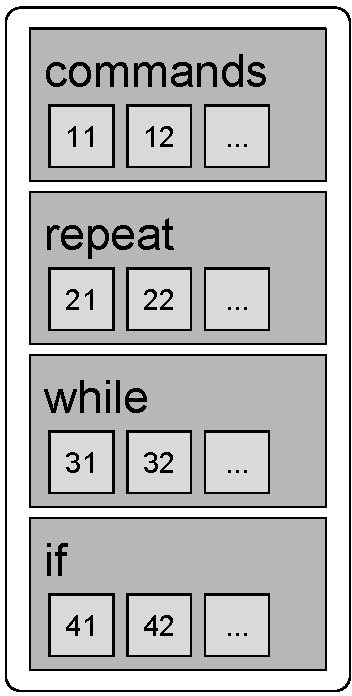
\includegraphics[height=45mm]{img/concepts-tasks-disjoint}
\caption{Disjoint sets}
\label{fig:concepts-tasks-disjoint}
\end{subfigure}%
\begin{subfigure}[t]{0.44\textwidth}
\centering
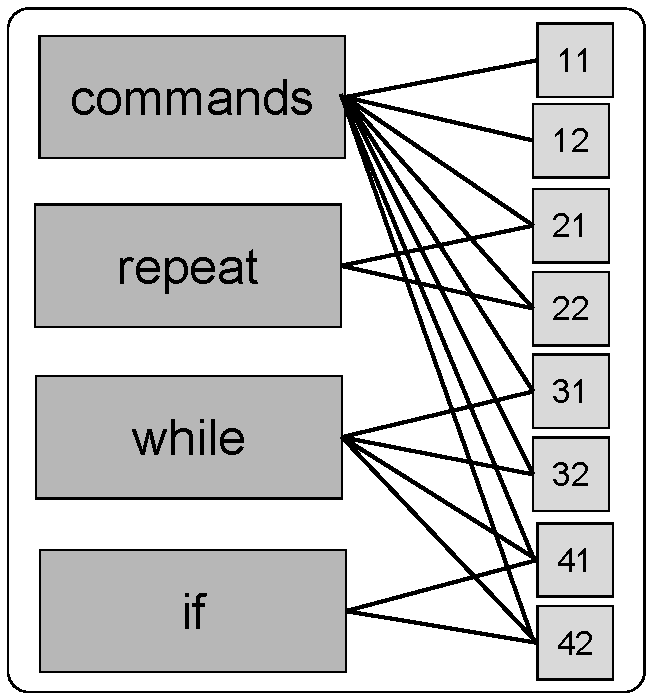
\includegraphics[height=45mm]{img/concepts-tasks-overlapping}
\caption{Overlapping concepts}
\label{fig:concepts-tasks-overlapping}
\end{subfigure}
\begin{subfigure}[t]{0.3\textwidth}
\centering
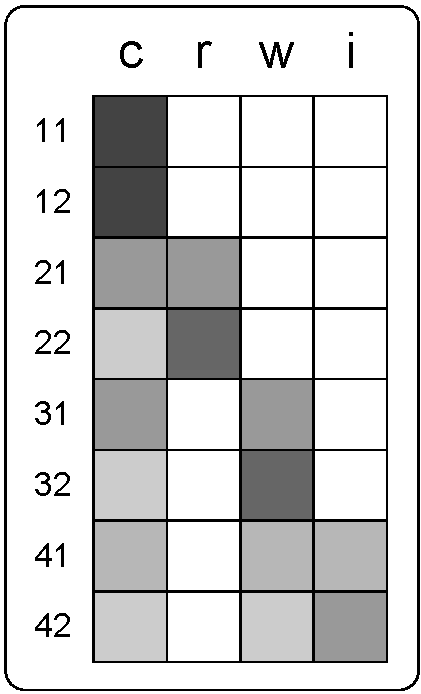
\includegraphics[height=45mm]{img/concepts-tasks-qmatrix}
\caption{Q-matrix}
\label{fig:concepts-tasks-qmatrix}
\end{subfigure}
\caption{%
  Relationship between tasks (light squares) and concepts (dark rectangles).
  Darkness in the Q-matrix shows strength of the relationship.} % TODO: grammar
\label{fig:concepts-tasks-relationships}
\end{figure}



%\imgW[0.8]{concepts-disjoint-overlapping}{%
%  %Comparison of disjoint and overlapping concepts.
%  In the disjoint model (left), each task belong to one concept,
%  while in the overlapping model (right), single task can contain multiple concepts.}
%
%\vspace{-25pt}
%
%\begin{figure}[htb]
%\centering
%\begin{subfigure}{.48\textwidth}
%\centering
%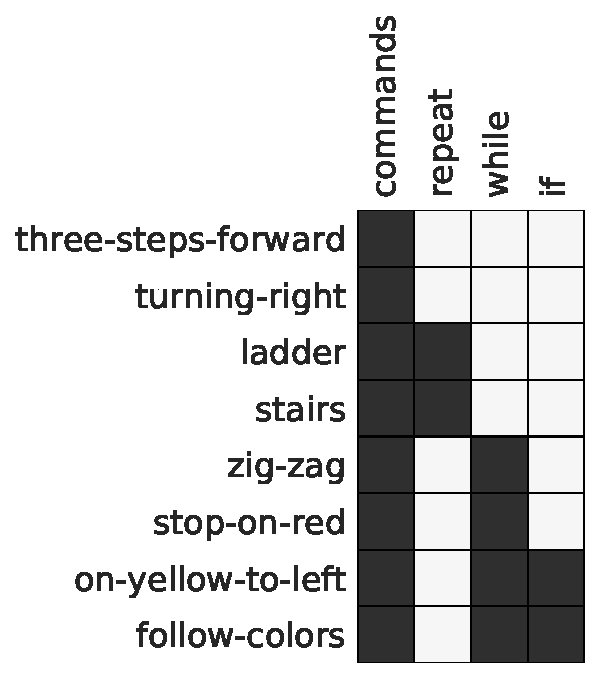
\includegraphics[width=0.65\textwidth]{img/qmatrix-binary}
%\end{subfigure}
%\begin{subfigure}{.48\textwidth}
%\centering
%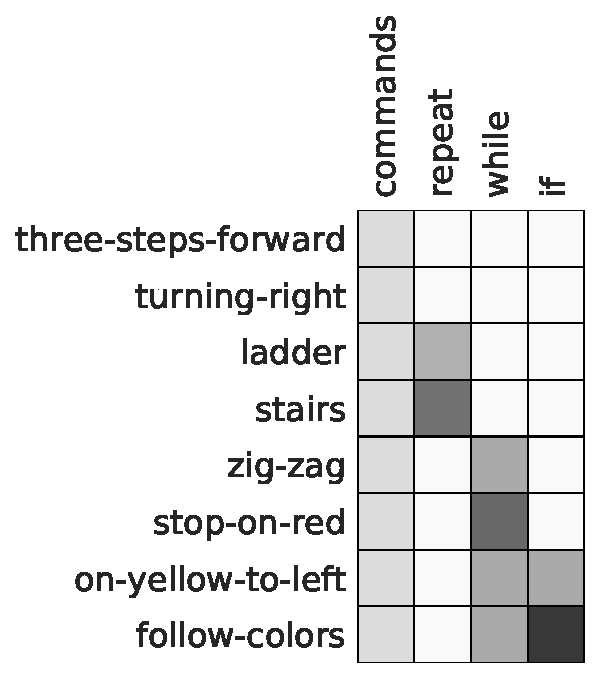
\includegraphics[width=0.65\textwidth]{img/qmatrix-continuous}
%\end{subfigure}
%\caption{%
%  Binary and continuous Q-matrices corresponding to the
%  bipartite graph of overlapping concepts from \cref{fig:concepts-disjoint-overlapping}.}
%\label{fig:qmatrix}
%\end{figure}


Concepts can be either set manually, or detected automatically
% NOTE: Automatically: a clustering algoritm (e.g. k-means, k-medoids, spectral clustering)
% operating on task-features or task-task similarity matrix
% (REF: our paper about similarity of programming problems)
\cite{niznan-thesis, rihak-phd}. % TODO: spec.pages
To use collected data while keeping the interpretability of manually defined
concepts, automatic techniques can be used to suggest small improvements to the
current tasks to concepts mapping \cite[chapter 3]{its-domain-models}.


%Manually defined concepts are interpretable and do not require collected data,
%but may be suboptimal for the intended usage of the domain model.
%%  so they can be used for skills visualizations in the user interface
%%  to provide students with the information about their learning progress.
%To combine advantages of both approaches, ALS can start with expert-provided
%concepts and later use automatic techniques to suggest how to improve
%the mapping from tasks to concepts \cite[chapter 3]{its-domain-models}.

%TODO: note on more complicated semantics of edges in the overlapping model,
%and assumptions leading to reduction of number of modeled parameters
%(e.g. conjunctive or conmpensatory concepts).


%\begin{itemize}
%\item (motivation) The assumption of a single concept for all tasks is
%  reasonable for many logic puzzles (e.g. sudoku), but not in programming.
%  For example, it is possible to master loops while struggling with functions,
%  and vice versa.
%\item TODO: define/REF
%\item aka knowledge components \cite{knowledge-components}
%\item granularity: while-loop < loops < programming
%\item modeling decisions: which concepts, how granular, what are the
%  relationships between them, which tasks belong to which concepts?
%\end{itemize}

%KLI framework \cite{kli-framework}, KCs with examples for programming:
%- variable-variable (principle):
%  - very coarse: programming
%  - coarse: loops
%  - medium: while loops
%  - fine: programs with a single while-not-end loop
%- variable-constant (category):
%  - coarse: game elements and mechanics?
%  - medium: asteroid?, winning rule?
%  - fine: ?
%- constant-constant (fact):
%  (names of game elements / names of parts of the environemnt / names of programming blocks),
%  (behavior of game elements, e.g. what happend when you hit the asteroid)

%\subsubsection{\textbf{Disjoint Concepts}}
%\begin{itemize}
%\item task:concepts 1:m (each task in execatly 1 concept)
%\item aka "concept model", "flat concepts" (concepts are flat clusters of tasks)
%\item Concepts can be either defined manually or detected automatically
%  (REF: \cite{niznan-thesis, rihak-phd}, spec.pages),
%\item automatically: a clustering algoritm (e.g. k-means, k-medoids, spectral clustering)
%  operating on task-features or task-task similarity matrix
%  (REF: our paper about similarity of programming problems)
%\item or semiautomatically, improving upon a mapping from tasks to concepts
%    provided by an expert \cite{its-domain-models}, chapter 3).
%\item Manually selected concepts, such as loops and conditional commands,
%  have the advantage of being interpretable,
%  so they can be used for skills visualizations in the user interface
%  to provide students with the information about their learning progress.
%  Furthermore, no data needs to be collected in advance,
%  while the automatic techniques require a lot of data to provide stable results.
%  (TODO: specify "a lot of" + REF).
%\item example in \cref{fig:concepts-disjoint-overlapping} (left)
%\item REF: usage (? ProSo - single concept per problem type, e.g. all tasks in Robotanist are single concept)
%\end{itemize}
%
%\subsubsection{\textbf{Overlapping Concepts}}
%\begin{itemize}
%\item (motivation) Single programming task may require multiple skills
%  at once, e.g. both loops and conditional commands (REF to figure with such task).
%\item task:concepts m:n (i.e. each task can contain to multiple concepts)
%\item represenation: bipartite graph between tasks and concepts
%  (example in right part of \cref{fig:concepts-disjoint-overlapping})
%\item another representation: matrix tasks x concepts -> 1 if contained, 0 if
%  not = "Q-matrix" (see \cref{fig:qmatrix})
%\item values: binary (hard containment) / continuous (soft containment --
%  how much is given concept important for given task; concepts are fuzzy sets of tasks)
%\item Q-matrix is a special type of feature matrix, where all features correpond to concepts
%  (and the values are normalized)
%\item constructing Q-matrix: manually vs. automatically
%  (disadvantage of automatic approach is that it requires quite lot of data and
%    that the discovered concepts are not-interpretable) (TODO: REF)
%\item human-in-the-loop approach: does existing Q-matrix (possibly created by
%  expert) match collected performance data? what to change for better fit?
%    (small "safe" improvements)
%%\item tradeoff between plausibility and complexity:
%%  having multiple concepts per tasks introduces "credit assignement problem"
%%  = "Which concept is responsible for poor performance?"
%%  (details in \cite{pelanek-learner-modeling} + TODO: spec. page)
%\item semantics of the edges is now more complicated than for disjoint concepts,
%  because each concept can be presented in the task to a different degree
%  and skills in these concepts may interact in diverse ways,
%  (?) generally: any function mapping the skills (or their probability
%    distributions) of the parent concepts to the predicted performance (or its
%    probability distribution) (e.g. in general BN);
%\item usually, some assumptions are made to decrease the number of modeled parameters;
%  for example:
%    additive model (skills are added, so a higher skill can compensate for a lower skill),
%    conjunctive model (all skills needed to solve the task)
%    disjunctive model (any single skill is enough),
%    DINA and DINO (which are probabilistic versions of conjuctive and disjunctive modes
%    respectively, that introduce a \emph{guess} and \emph{slip} factors to give a nonzero
%    probability to the events such as when a student solves a task without
%    having mastered all required skills).
%    \cite[chapter 3]{its-domain-models}.
%\item Additive models can also include a normalization of the sum, e.g.:
%  $\hat{p}_{ij} = \sigma(s_j \cdot t_i)$, where
%  $\hat{p}_{ij}$ is the predicted (continuous) performance of student $j$ on task $i$,
%  $s_j$ is the vector of skills, $t_i$ is the row in Q-matrix for the task $i$,
%  and $\sigma$ is logistic sigmoid. (TODO?: example)
%  (TODO: fix: performance is undefined at this point...)
%% TODO: consider precise formulation for all other models as well,
%% see \cite[chapter 3]{its-domain-models}.
%% Note: We can also look on the interpretation from the other side: once the task
%% is failed, which skill(s) is/are to blame and how much (ie. how to decrease our estimates
%% if we predicted a success).
%\item TODO: is there an interpretation makes best sense in our domain?
%  (DINA and additive models seem reasonable, others not;
%  TODO: add an example to illustrate why the others are bad for us).
%\end{itemize}


%\subsection{Problem Sets}
%
%\begin{itemize}
%\item aka task sets, topics, units, chapters,
%  (and we call them "missions" and "mission phases" in RoboMission)
%\item ? usually corresponds to concepts (or it is convenient if they do),
%\item can be hierarchical (and the hierarchy should match the hierarchy of
%  corresponding concepts)
%\item can be ordered (and the ordering should follow the prerequisity structure
%  of corresponding concepts)
%\item single concept can be practiced by multiple problem sets
%  (e.g. loops in robot on grid and in turtle graphics)
%\item usually presented in the UI (? so it can be viewed as a part of the UI model instead)
%\item REF usage: everywhere (Umime programovat, Tutor -> Robotanist is a single PS)
%\item TODO: discuss example of Umime programovat (tree of concepts, problem
%  sets, each PS maps to a (single?) concept; where are items?)
%\end{itemize}


\subsection{Hierarchical Models}

Concepts vary in granularity and create hierarchies.
For example, programming concept include loops, loops include while loops,
and while loops include programs with a single while-not-end loop.
% TODO: CITE \cite{kli-framework}?
Hierarchy can be modeled either as a rooted tree (single parent concept allowed),
or as a directed acyclic graph (DAG) (\cref{fig:concepts-hierarchical}).
Although hierarchical concepts can be used without modeling the hierarchy
(using overlapping concepts, e.g. a task can contain while loops and
a more general loops concept), explicitly modeling the hierarchy of concepts in
the introductory programming can improve accuracy of the overlaying student model
\cite{learner-models-integration-skills}.
% NOTE: paper: they model domain as BN with 4
%types of nodes: observations, base concepts, integration concepts (TODO:
%example), cognitive load node; they show that it's important to have also
%tasks linked directly to these integration concepts.

%\imgW{concepts-hierarchical}{Hierarchial concepts as a tree (a), or a DAG (b).}

\begin{figure}[htb]
\centering
\begin{subfigure}[t]{0.4\textwidth}
\centering
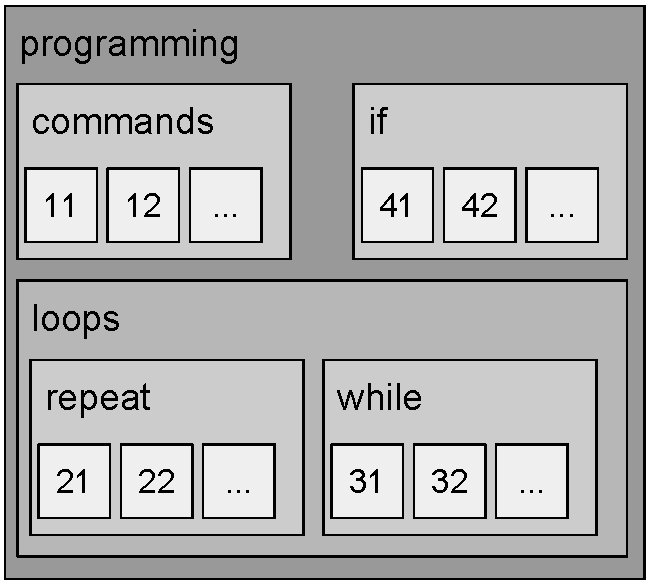
\includegraphics[height=45mm]{img/concepts-hierarchical-tree}
\caption{Tree of concepts}
\label{fig:concepts-hierarchical-tree}
\end{subfigure}%
\begin{subfigure}[t]{0.6\textwidth}
\centering
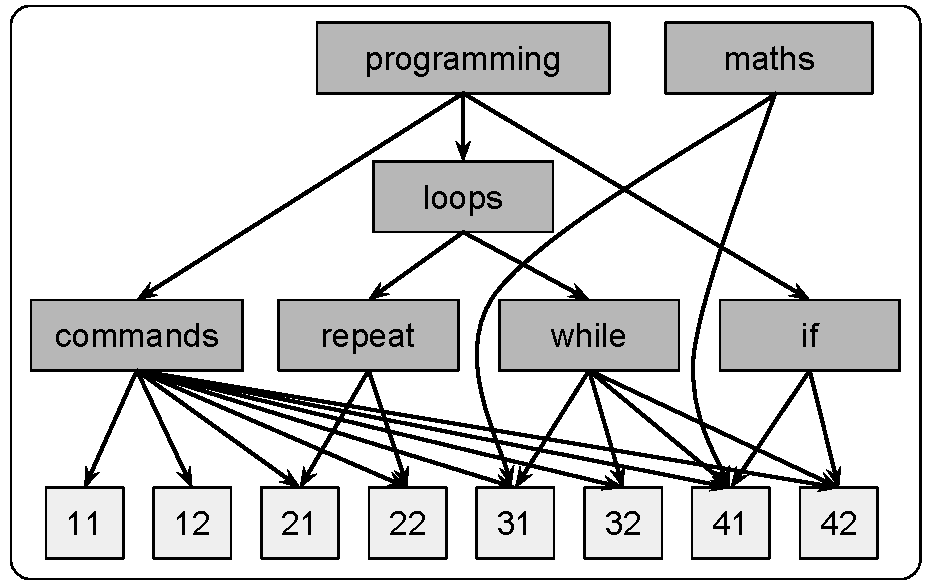
\includegraphics[height=45mm]{img/concepts-hierarchical-dag}
\caption{DAG of concepts}
\label{fig:concepts-hierarchical-dag}
\end{subfigure}
\caption{Hierarchical domain models.}
\label{fig:concepts-hierarchical}
\end{figure}

%\begin{itemize}
%\item in addition to the relationships between tasks and concepts,
%  we can also model the relationships between concepts
%\item two commonly modelled relationships are generalization (this section) and
%  prerequisities (next section)
%\item hierarchical model = allow for generalization relationship between concepts
%\item (relationship name: generalization / specialization / inclusion ?)
%\item representation: rooted tree of chunks, inner nodes = concepts, leaves = tasks
%\item extension: DAG instead of tree
%  (comparision tree vs DAG in \cref{fig:concepts-hierarchical})
%\item Note that we can of course use hierarchical concepts and yet decide not to
%  model a hiearachy (although in that case, overlapping concepts are necessary,
%  e.g. if the task practices while loops, it also practices loops and programming concepts).
%\item construction: manually/automatically (hierarchical clustering?)
%\item TODO: discuss relationship between inclusion and prerequisities
%  (Q: isn't inclusion just a special case of soft prerequisity?
%  You need to master loops before you master programming (AND-node),
%  you need to master at least one of these tasks to master the loop concept (OR-node).)
%\item REF usage: MatMat (math domain)
%\item tasks in leaves only / in all nodes (different semantics of inner nodes:
%  "composition of independent concepts" vs "integration concepts"
%\item Experiment showing usefulness of hierarchial model in introductory programming:
%  \cite{learner-models-integration-skills} -- they model domain as BN with 4
%    types of nodes: observations, base concepts, integration concepts (TODO:
%    example), cognitive load node; they show that it's important to have also
%    tasks linked directly to these integration concepts.
%\end{itemize}


\subsection{Prerequisites}

Prerequisites specify which learning objects need to mastered prior to
tackling a given learning object.
For example, single loop is a prerequisite for nested loops.
% If learning objects has multiple prerequisites, there are two common interpretations:
There are two common interpretations of multiple prerequisites:
\emph{conjunctive prerequisites} (all must be be mastered)
and \emph{disjunctive prerequisites} (one mastered is enough).
Conjunctive and disjunctive prerequisites can be represented together by
\emph{and-or graph} (\cref{fig:prerequisites-and-or}).
If only conjunctive prerequisites are needed, then it is enough to represent
prerequisites by a DAG, called \emph{Partial Order Knowledge Structure}
(POKS \cite{poks}, \cref{fig:prerequisites-poks}).
More generally, each learning object can specify a function from skills of
its prerequisites
into a prior skill (and leave the \emph{ready-to-tackle decision} on a tutor model).
If the skills can be interpreted as probabilities, then the resulting prerequisite structure
is a \emph{Bayesian network}; this approach was used in \cite{its-programming}.
% TODO: CITE BN.
% NOTE: its-programming: prerequ. between concepts interpreted as BN (params
% computed from historical data);

%\imgW[0.9]{chunks-prerequisites}{%
%  Left: prerequisites between first-level concepts (AND);
%  right: prerequisites between tasks (AND-OR).
%  TODO: "while+if-else"; add separate and-nodes and use arc for ANDs instead of ORs}

\begin{figure}[htb]
\centering
\begin{subfigure}[t]{0.45\textwidth}
\centering
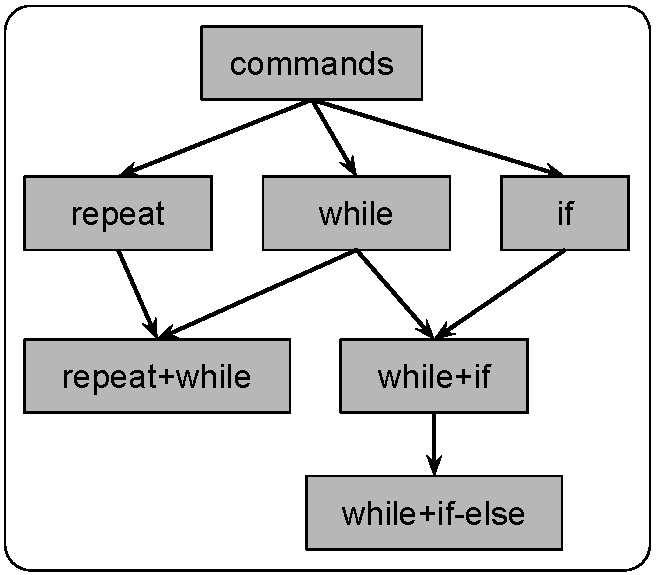
\includegraphics[height=40mm]{img/prerequisites-poks}
\caption{POKS of concepts}
\label{fig:prerequisites-poks}
\end{subfigure}%
\begin{subfigure}[t]{0.55\textwidth}
\centering
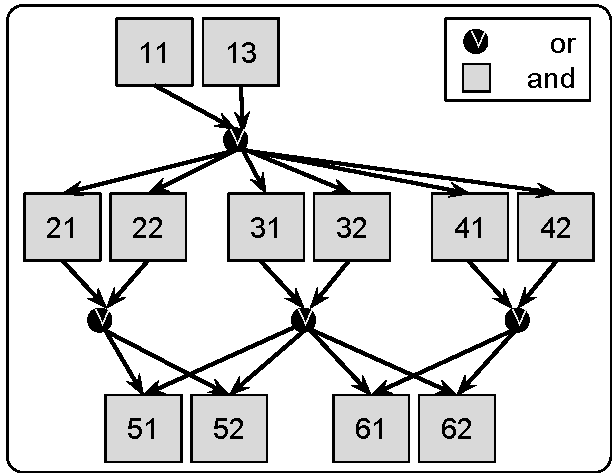
\includegraphics[height=40mm]{img/prerequisites-and-or}
\caption{And-Or graph of tasks}
\label{fig:prerequisites-and-or}
\end{subfigure}
\caption{Domain models with prerequisites.}
\label{fig:chunks-prerequisites}
\end{figure}

%\begin{itemize}
%\item multiple edges -- multiple interpretations: e.g.:
%  AND (all prerequistes must be met),
%  OR (at least one prerequisity must be met),
%  (TODO?: noisy and, noisy or),
%  ? additive (compensatory) prerequisites
%  (analogous to the multiple concept skills to task performance mapping).
%\item Generally, the interpretation can be any function from skills/performance
%  associated with prerequisites to a (binary) decision whether the prerequisites are met
%  (when working with probabilities, this leads to Bayesian networks?)
%\item special case of only AND nodes = POKS ("Partial Order Knowledge Structure")
%\item representation: genarally BN, restricted: AND/OR directed acyclic graph (DAG),
%  or even just DAG for POKS (examples in \cref{fig:chunks-prerequisites})
%\item REF usage:
%  (1) KSI (existing systems) -- and/or prerequisities between tasks;
%  (2) \cite{its-programming} -- soft (continuous) prerequisities (and only?)
%    between concepts interpreted as BN (params computed from historical data);
%  (3) another example (for math): Dybuster Calcularis (Design and evaluation of the computer-based training program calcularis for enhancing numerical cognition.)
%\item can be combined with the hieararchical models
%  (?) and it can actually make the prerequisity structure easier, because
%    many edges between two groups of chunks on the same level
%    can be replaced by a single prerequisity between 2 higher-order chunks
%    (this is an example of the inheritence property).
%  (TODO: picture to illustrate the point, showing how many prerequisites between
%    2 groups of tasks can be replaced by a single prerequisity edge between 2 concepts)
%\end{itemize}


\subsection{Similarities}

%Similarity is a symmetric relationship between learning objects of the same type, for example tasks.
Similarities can be represented either as a matrix of values from range $[0, 1]$
(the higher number, the more similar objects),
or as a graph with edges between the most similar learning objects
(\cref{fig:similarities-tasks}).
In the \emph{network model} \cite{rihak-phd}, task similarities are used to propagate
knowledge about one task (observed performance) to another tasks (estimated performance)
directly, without using concepts.
% example: if student solves a task -> update our performance estimates on all other tasks
The most important decision when computing similarities is what data to use.
The decision depends both on the intended usage and on the amount of collected data
available. For example, performance data are useful if the similarities are used in a
student model to predict future performance; however, it requires that enough
performance data is collected in order for the computed similarities to be stable.
%Similarities between tasks, can be computed from either a feature matrix using task settings and solutions,
% NOTE: 2nd level of similarity - often helps (when using performance data) \cite{rihak-phd}
% REF: to our research on item similarity in introductory programming
%(TODO: mention the most relevant results from the paper:
% which data to use -- important, which metric -- less important; recommended transformations)
% TODO: CITE some papers on computing similarities (e.g. our paper)

\begin{figure}[htb]
\centering
\begin{subfigure}[t]{.48\textwidth}
\centering
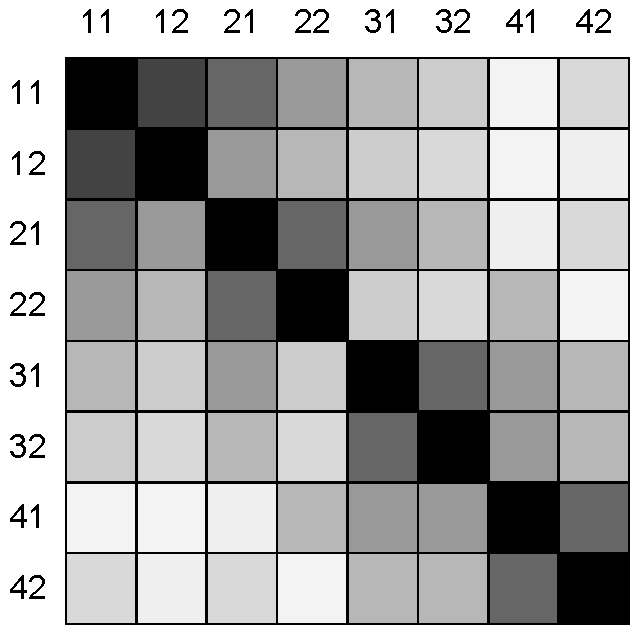
\includegraphics[width=0.7\textwidth]{img/similarity-matrix}
\caption{Similarity matrix}
\end{subfigure}
\begin{subfigure}[t]{.48\textwidth}
\centering
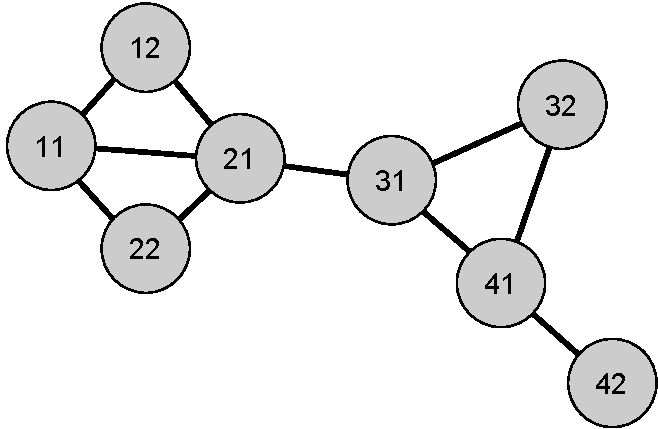
\includegraphics[width=0.8\textwidth]{img/similarity-graph}
\caption{Similarity graph}
\end{subfigure}
\caption{%
  Representation of soft and hard similarities between tasks.}
\label{fig:similarities-tasks}
\end{figure}


%\subsection{Evaluation}
%
%\begin{itemize}
%\item problem: many options, which one to choose
%\item again: no single best domain model depends on its intended usage
%\item thus: the model should be evaluated wrt. the usage,
%  which can mean we can reduce the problem of evaluation the domain model
%  to the evaluation of the application -- try a bunch of different domain
%  models and see their effect on the performance in the application
%\item limitations:
%  (1) Only works with a small number of domain models to try
%  (if we want to optimize a continous parameters of the domain, then it
%    is more difficult).
%  (2) Requires the ability to evaluate the application, which is not
%    always possible (e.g.: getting insight, open learner model) or is
%    slow (e.g. requires online experiment).
%\item REF to details on evaluation in the last sections of this chapter
%\item TODO: illustrate: select one example of evalution and describe properly
%  (some approaches to evalution are e.g. in \cite{rihak-phd})
%\item TODO: example -- learning curve analysis \cite{its-domain-models}
%\item example: verification of homogeneity of tasks that are assumed to be
%  homogenous (interchangeable) according to current model (ie. they should
%  have similar average success and solving times; statistical test testing
%  that solving times comes from different distributions can be performed)
%  (TODO: perform such test and illustrate, showing the two distributions
%  and result of the test)
%\end{itemize}



\section{Student Modeling}
\label{sec:student-modeling}

Student model captures state of the student (e.g. skills) estimated from the
past performance. Usually, it enables to predict future performance
%Comprehensive overviews of student modeling:
\cite{its-learner-models, student-models-review-2012, pelanek-learner-modeling}.
It is used in tutor models to detect mastery, or to select tasks matching
student's skills, in the user interface to visualize skills \cite{instructor-dashboard-realtime},
and in the analyses to get insight into how the students are learning.  % TODO: elaborate
% TODO: add citations of examples for usages

% NOTE: in tutor models += showing hints when a student is digressing from the
% path towards a solution.
% NOTE: In UI: showing feedback for the students and teachers
%        (visualization of skills -- "open learner model").


%\subsection{Domain vs. Student}
%
%TODO: These are just internal notes. After incorporate clarifying comments
%to relevant places, consider removing this section.
%
%\begin{itemize}
%\item The line between "domain" and "student" is fuzzy.
%  It differs a lot in different papers; some even don't distinguish a separated
%  domain model. (REF examples)
%\item We have decided to take the following approach:
%  The sole responsibility of student model is to track skills of a \emph{single}
%  student. Thus, the domain model includes also population-specific parameters,
%  such as initial skills, learning rate, chunk difficulties,
%  precise (numeric) relationships between skills (prerequisites, mastery).
%\item ?? Some of these parameters are learned within the domain model
%  and then used as fixed parameters in the student model.
%\item TODO: The above notes about population parameters to the domain section.
%\item We could define a separate \emph{population model}, which would be useful
% if ?? we would like to model more populations and/or
% estimate the population parameters online
% (?? REF: slepe mapy - prior knowledge + difficulties estimation)
%\item Note that even which chunks exist what are the relationships between them
%  may depend on the population (if the population is diverse), so there is
%  really no clear division on what should be a part of
%  "population independent domain model" and "population model"
%  (because it inherently depends on the population using the system,
%  so we can decide only for the current population and provided we have collected
%  enought data to analyze how large the differnces between subpopulations are
%  and if it has significant impact on the application the model is used for).
%\item ?? While being non-standard, we found this division to best match separation
%  of concerns and thus be suitable for both explaining (as in this text)
%  and impelementation (as in the developed system).
%\item Domain vs Student:
%  initial skills x current skills,
%  concepts x skills,
%  (tasks x performance),
%  difficulties x skills,
%  common for all students x for each student,
%  offline x online.
%\item Domain = state space, student = point in that space space
%  (\cite{its-learner-models}).
%\item example (from \cite{its-programming}):
%  domain model is DAG of concepts together with a Bayesian network over this DAG
%  (i.e. assignment of conditional probabilities to the edges),
%  student model is (for each student) assignment from each concept to the
%  knowledge (known / unknown / not-sure) -> knowlege for any concept can be
%  then inferred using the Bayesian network.
%\end{itemize}


\subsection{Classification of Student Models}

\begin{itemize}
\item \emph{Modeled components.}
In addition to modeling skills, broader student models can also
include emotions (e.g. frustration, boredom), needs, preferences, motivation,
and metacognition \cite[ch.\,10]{affect-sensor-free,its-review-2010}.
%(knowledge about their knowledge) (REF).
% NOTE: + preferences, e.g. about ideal challenge level, amount of text, theme,
% e.g. prefer tasks with a shooting spaceship or with ice-skating princesses
\item \emph{Underlying domain model.}
The simplest models assume a single concept,
% or each task as separate concept. %(REF: slepe-mapy).
more complex models can include multiple concepts,
hierarchies, prerequisites, or similarities (\cref{sec:domain-modeling}).
\item \emph{Granularity of modeled events.}
Some models track the state of the student during solving a task
\cite{bkt, sqltutor}, % TODO:CITE: rule-based models, constraint based models),
while others describe the state of the student only between tasks %sessions
\cite{kli-framework}. % TODO: check, add citation
% or even only between finished problem sets.
\item \emph{Discrete or continuous skills.}
Some models assume discrete skills (e.g. known, or now know, or with multiple levels),
% e.g. unknown -> known -> fluent; or LogisticHMM
%(CITE/REF:BKT)
while others assume continuous skill
%(CITE/REF: logistic models).
\cite{pelanek-learner-modeling}.
\item \emph{Representation of skill estimate.}
Instead of modeling full probability distribution of the skill, % discretized?
most models track only a single point estimate
(possibly with another parameter describing its uncertainty).
% TODO:CITE?
%?? or they assume a specific shape of the distribution that can be described by
%a few numbers (e.g. mean and standard deviation for normal distribution).
\item \emph{Representation of performance}.
  Binary correctness (solved or failed),
  discrete performance levels (e.g., poor, good, and excellent),
  continuous performance (in range $[0, 1]$),
  %(\emph{partial credit} CITE) ($p_{ij} \in [0, 1]$)
  or solving time.
  %log-time (REF: why log; possibly also REF to a relevant figure in Analysis chapter),
% NOTE:score combining time and correctness \cite[p.106]{rihak-phd} -- not relevant for use
%\item ?? \emph{probabilistic models} (vs. deterministic)
%  = predict a probability distribution of performance instead of a single point
%  (?? and/or represent skill as probabilist distributions?)
\item \emph{Predictive or descriptive}.
Predictive models can predict the performance of the student on a given task,
while descriptive models only summarize the past performance of the student.
% TODO:CITE/example (NCC)
\item \emph{Online or offline.}
In online models, parameters can be updated gradually after each task session
(i.e. there exist an efficient online algorithm for learning model parameters).
% CITE: online algorithms.
\item \emph{Assumptions about learning.}
Models used in \emph{adaptive testing} \cite{cat} assume no learning.
%during interaction with the system.
%They can be reduced to models with
%learning by reestimating skills from the full student history after each task
%session, but this leads to offline models.
Models that include learning use additional assumptions
about how the learning happens. % TODO:CITE:examples
% e.g. a constant increase of skill after each attempted task (CITE:PFA?).
%For example, BKT (\cref{sec:bkt}) assumes a discrete transtion from unknown
%state to the known state.
%\item \emph{Complexity} (\cite{pelanek-learner-modeling} + TODO:page)
%The more skills and relationships between them the model includes,
%the more precisely it can capture the reality, but only
%if there is enough data to train the model; otherwise we are in danger of
%overfitting. (TODO: REF to the bias-variance tradeoff).
%The number of parameters that are specific for students must be low in order to
%estimate them quickly after just a few interactions of the student with the system.
%(+ they are assumed to change, no older observations loose their value)
%More complex models might be also more difficult to implement, debug and interpret.
%   (?? this is a different kind of complexity; the first is size of hypothesis space)
\end{itemize}

%Which student model to used depends on the domain, intended usage, and also
%on the type and amount of data we have.
%In the rest of this section, we restrict our attention to the models relevant
%for the domain of introductory programming and the type of the system we
%are building. Specifically, we focus on models that
%model only skills of concepts and predict performance on tasks,
%allow for multiple skills per task,
%assume learning and can be updated online.

In \cref{sec:logistic-models,sec:dbn}, we describe two broad
families of predictive models of a student between tasks,
focusing on their versions % suitable for ALS for learning programming,
that can incorporate multiple concepts, learning and allow for online update. % of parameters.

\subsection{Skills and Performance}
%\subsection{Data and Algorithms}

Student model use a domain model as an underlying structure,
assigning estimated \emph{skills} to each concept, % either estimated or self-declared
and \emph{performances} (either observed or predicted) to each task.
% NOTE: space-time tradeoof: Typically, all but the predicted performances are stored.
%Skills can be represented as a single point estimage, or with uncertainty,
%  or even full distribution of the estimated skill.
Similarly as skills summarize all previous task sessions of the student,
performance is a compressed information about the series of
interactions with the task (code edits, executions, taken hints, user rating). %self-evaluation).
Performance compression can range from simple heuristics based on summary statistics
(e.g. specifying solving time thresholds for excellent and for good performance),
through more complex algorithms that would consider all interactions with the task,
to a recurrent neural network reading the series
of program snapshots embeddings  % AST transformed to vectors of floats
\cite{student-models-deep-learning}.
% NOTE: Sweat spot: somewhere in between these two rather extreme approaches.

While the compression causes a loss of information, it also reduces noise
present in the raw data. Moreover, it helps to avoid a combinatoric
explosion of considering each type of model with multiple different types of
input data and their combinations.
The most important consideration for performance compression is what data
(correctness, solving time, etc.) to use \cite{alg.mastery}.
%Used data play an important role, e.g. in \cite{alg.mastery}
%Having a unified simple performance input makes the models simpler and easier to interpret.
%Used data play an important role, e.g. in \cite{alg.mastery} they achieved
%better results in mastery learning by incorporating solving times into the
%performance instead of using just binary correctness (TODO: domains? math,
%czech).

% EXT:
%There are three types of algorithms linked to student models: online update
%of skills after a new task session, prediction of performance on given task,
%and insight algorithms that work either with a single student (e.g. skills
%visualization), or a population (e.g. plotting learning curves).



%\subsection{Performance}

%\begin{itemize}
%\item Observed data from a task session:
%  solved/not, solving time, number of code executions, number of edits,
%  or even the individual edits (program snapshot), hints taken,
%  rating or labels provided by the student (e.g. perceived difficulty).
%\item TODO: mention different granularity/frequency levels for taking program
%  snapshots: edits (AST changes), executions
%  (REF: Educational Data Mining and Learning Analytics in Programming:
%  Literature Review and Case Studies -- they differentiate more levels:
%  and instead of "AST changes" they specify 2 levels ("key strokes" and
%  "line-level edits"), but only the two are relevant for us (and most online,
%  block-base programming environmant).
%\item We first compress these \emph{observational data} into a
%  single number representation of \emph{performance}.
%\item The chosen representation/computation may play important role for the usage
%  of the student model, e.g. in \cite{alg.mastery} they achieved better results
%  in mastery learning by incorporating solving times into the performance instead
%  of using just binary correctness (?? domains: math, czech).
%\item Performance representation in introductory programming:
%  most students solve most tasks given enough time, so correctness is out of
%  question. We could still map task session data into a binary performance (1
%  = good, 0 = poor), but that would not allow to distinguish between students
%  for whom are the tasks just right and those for whom are too easy.
%\item Three-level domain $p_{ij} \in \{0, 0.5, 1\}$ (poor, good, excellent performance)
%  could already contain sufficient information for many applications
%  (should be verified by future research)
%  and matches the predictions whether a given task is for given student too
%  difficult, just right, or too easy.
%\item Ordinal scale from definition;
%  ??  It is convenient to treat it as an interval variable,
%  but then it should be verified on data that the chosen compressed performance
%  behaves accordingly. (TODO: explain / REF to a paper or relevant analysis in
%  thesis)
%\item ?? range $[0, 1]$ vs. -1, 0, 1; (disadvantage of 0-1: suggest it has interval
%  scale + possible confusion with the probabilistic interpretation, which
%  doesn't make much sense -- unless we assume a very specific shape of the
%  probablistic distribution, we need to specify 2 numbers to get the probablity
%  table)
%\item Example of performance compression/extraction:
%  based on solving time thresholds
%  (e.g., $0.5 \times \text{median}$, $2 \times \text{median}$)
%  (+ possibly REF other examples)
%  (??TODO: figure -- with multiple possible representations).
%\item The compression algorithm can be much more complex;
%  for example, a trained recurrent neural network reading a series
%  of program snapshots embeddings  % AST transformed to vectors of floats
%  \cite{student-models-deep-learning}.
%\item Another option would be to model log-times (used e.g. in Tutor - REF),
%  or continuous partial credit by mapping solving times to the 0-1 range
%  (e.g linear fn from 0s to 2*median secs, then 0 \cite{alg.mastery}).
%\item While the compression causes a loss of information,
%  it also reduces noise present in the raw data.
%  Most importantly, it helps to avoid a combinatoric explosion of
%  considering each type of model with multiple different types of input data or
%  their combination.
%  Having a unified simple performance input makes the models simpler and
%  easier to interpret.
%\item Notation: true performance $p_{ij}$ vs. predicted performance $\hat{p}_{ij}$
%\end{itemize}


%\subsection{Skills}

%\begin{itemize}
%\item (domain vs. student: tasks -- performance, concepts -- skills)
%\item ?? definition:
%  $\theta_{cj} \in [0, 1]$ expresses how much student $j$ knows concept $c$
%  (0 not at all, 1 mastered).
%  (?? TODO: Consider using $[-1, 1]$ with 0 calibrated either to the "ready-to-learn"
%  concept (flow point), or to the initial student.)
%\item Possibly: not only a single point estimage, but also uncertainty,
%  or even full distribution of the estimated skill.
%\item Note: terms "skills" are often used interchangebly with "concepts" in
%  the literature; in this thesis we strictly distinguish between "concepts"
%  (independent of any student) and "skills" (associated with a student-concept
%  pair).
%\item Each student model thus depends ("overlays") a domain model, which
%  defines a set of concepts for which to associate skills
%  and describes how these skills interact among themselves and how they
%  relate to each task.
%\item Student models use domain as a structure,
%  assigning skills (and possibly other parameters, such as uncertainty)
%  to the chunks in that structure.
%\end{itemize}


%\subsection{Data and Algorithms}

%We specify the model by its data and procedures
%(as in \cite{pelanek-learner-modeling}).
%We further distinguish between the historical data that are transformed into
%the model data (by an online update function after each task session).
%
%\subsubsection{Historical Data}
%\begin{itemize}
%\item list of task sessions
%\item task session is $(t, i, j, c, p^{t}_{ij})$ with
%  timestamp $t$ , task $i$, student $j$, (context $c$),
%  observed performance $p^{t}_{ij}$.
%\end{itemize}
%
%\subsubsection{Model Data}
%\begin{itemize}
%\item underalying domain (e.g. disjunctive concepts),
%\item population parameters, e.g. initial skills, learning rate,
%\item skills for each student-??concept pair.
%\end{itemize}
%
%\subsubsection{Algorithms}
%\begin{itemize}
%\item \emph{learning} population parameters (can be offline),
%  (?? can we make population parameters part of the domain to have a single
%  group of "offline-learned" parameters = domain = everything independent
%  of a specific student)
%\item \emph{update} of student skills based on an observed task session
%  (online learning),
%\item \emph{prediction} of performance for given student and task.
%  (?? also prediction of skill for student-concept,
%  if the data are more complex, e.g. hierarchical model?),
%\item \emph{visualization} of a group of learners, e.g. learning curves
%  (?? broader -- insight: also clustering of students, ...)
%\item TODO: figure showing interaction between the data and algorithms.
%\end{itemize}
%
%\subsubsection{Learning population parameters}
%\begin{itemize}
%\item input: domain $D$, history: collected task sessions
%\item output: population parameters $P$: initial skills, learning rate, ...
%\item TODO: replace text by a figure
%\end{itemize}
%
%\subsubsection{Online skill update}
%\begin{itemize}
%\item input: domain $D$, (population parameters $P$),
%  student state before the task session $\theta^{t}_{j}$,
%  new task session $(t, i, j, p^{t}_{ij})$
%\item output: student state (skills) after the task session $\theta^{t+1}_{j}$
%\item TODO: replace text be a figure
%\end{itemize}
%
%\subsubsection{Performance prediction}
%\begin{itemize}
%\item input: domain $D$, (?? population parameters $P$),
%  student state $\theta^{t}_{j}$, task $i$, (context)
%\item output: predicted response of the student to the task,
%  e.g. performance $\hat{p}^t_{ij}$
%\item TODO: replace text be a figure
%\end{itemize}


\subsection{Logistic Models}  % OR "Elo models"
\label{sec:logistic-models}

Logistic model \cite{irt-visual-guide}  % TODO:check-cite
predicts performance $P(s, d)$
of a student with skill $s$ on a task with difficulty $d$
using a logistic function applied to the difference between the skill and the difficulty (\cref{fig:logistic-model}).

\begin{figure}[htb]
\centering
\begin{subfigure}{.58\textwidth}
\centering
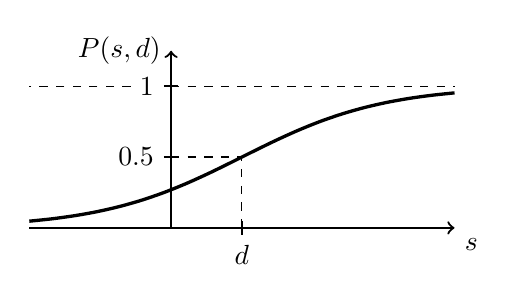
\begin{tikzpicture}[domain=-2:4, smooth, samples=20, scale=0.9]
\draw [thick, ->] (-2,0) -- (4,0) node [below right] {$s$};
\draw [thick, ->] (0,0) -- (0,2.5) node [left] {$P(s,d)$};
\draw [thick] (-0.1,1) node [left] {$0.5$} -- (0.1,1);
\draw [thick] (-0.1,2) node [left] {$1$} -- (0.1,2);
\draw [thin, dashed] (0,2) -- (4,2);
\draw [thin, dashed] (0,1) -- (1,1) -- (1, 0);
\draw [thin, dashed] (-0.57,2) -- (-2,2);
\draw [thick] (1,0.1) -- (1,-0.1) node [below] {$d$};
\draw [very thick] plot (\x, {2 / (1 + exp(1 - \x))});
\end{tikzpicture}
\end{subfigure}
\begin{subfigure}{.38\textwidth}
\centering
\begin{equation}\label{eq:logistic}
P(s, d) = \frac{1}{1 + e^{-(s - d)}}
\end{equation}
\end{subfigure}
\caption{One-parameter unidimensional logistic model.}
\label{fig:logistic-model}
\end{figure}


Elo model \cite{alg.elo, mathsgarden} extends the logistic model
  to capture changing knowledge.
Inspired by the rating of chess players \cite{elo-rating},
  the model interprets each attempt  to solve a task
  as a match between the student and the task.
After this match ends, skill and difficulty estimates are revised.
Depending on whether the student solves the task better or worse than expected
  by the model, her skill is increased or decreased.
The size of the change is proportional to the prediction error, which is the difference
  between the predicted and the actual performance ($p_{ij} - \hat{p}_{ij}$). % (``surprise'').
  Elo can be further extended to utilize more complex domain models,
  such as multiple concepts with a hierarchy,
  or similarities between tasks \cite{rihak-phd}.
% TODO: explore and cite more extensions
%There are variants of Elo that work with more complex domain models,
%such as \emph{Multiple Skills Elo} for multiple disjoint concepts,
%\emph{Hierarchical Elo} for tree hierarchical model,
%and \emph{Network Elo} that utilize task similarities of the network domain model
%\cite{rihak-phd}.


%There are variants of Elo that work with more complex domain models,
%such as \emph{Multiple Skills Elo} for multiple disjoint concepts,
%\emph{Hierarchical Elo} for tree hierarchical model,
%and \emph{Network Elo} that utilize task similarities of the network domain model
%\cite{rihak-phd}.
%(TODO: what about overlapping concepts, which we are most interested in?)


%\begin{itemize}
%\item learning rate -- not decreasing, because the skill is assumed to change over time
%  (``nonstationary variable'')
%  \cite{student-models-recent-data}
%  % TODO: check the cited paper properly
%\item note: possibility to also update task difficulties online (with
%  decreasing learning rate, because the difficulties are assumed to converge)
%\item The main advantage of using the Elo model is its simplicity, flexibility (TODO: elaborate),
%  good prediction performance (REF) and intrinsic online nature, which allows for immediate
%  updates of parameters as students are interacting with the system.
%\item TODO: ?? relationship to PFA, PFAE
%\item The performance predicton and udpate depends on the underlaying domain model.
%  In the following sections, we discuss some of the possibilities.
%\end{itemize}
%
%\subsubsection{Single Skill Elo}
%
%\begin{itemize}
%\item underlying model: concept-free (REF)
%\item TODO: formulas (?? predicting what -- continuous partial score?)
%\item TODO: figure
%\item TODO: relationship to EMA
%\end{itemize}
%
%
%
%\subsubsection{Multiple Skills Elo}
%
%\begin{itemize}
%\item underlying model: Disjoint Concepts / Overlapping Concepts (REF)
%\item Disjoint Skills: as basic Elo but the total skill is the sum of the
%global skill and concept skill (updating both the same way) (\cite{rihak-phd}, TODO: page).
%\item TODO: Overlapping Skills: ?? (derivation from chosen error measure -> formulas)
%\item alternative solution to the ``credit assignment problem'':
%  not to update the skills directly after a failure on a single task,
%  but first diagnose the issue - give the student tasks with only a subset of concepts,
%  to find the problematic concept for which the skill should be decreased
%  \cite{assistment-trasfer-models}
%\end{itemize}
%
%\subsubsection{Hierarchical Elo}
%
%\begin{itemize}
%\item underlying model: hierarchical model (REF)
%\item REF: \cite{rihak-phd} -- assuming disjoint concepts
%\item predictions: total skill = sum all ancestors skills
%\item update: all ancestors sequentialy (from the top-most), elo-like update
%\item TODO: formulas
%\end{itemize}
%
%
%\subsubsection{Network Elo}
%
%\begin{itemize}
%\item underlying model: network model (REF)
%\item REF: \cite{rihak-phd}
%\item each time a task is solved, update skill for all tasks according to the
%similarity to the one solved (this can be propably also done on the level of
%concepts, if we have a similarity network between concepts)
%\item TODO: formulas
%\end{itemize}



\subsection{Dynamic Bayesian Networks}
\label{sec:dbn}

Another family of student models is based on \emph{Bayesian networks} \cite{probabilistic-ai},
in which nodes correspond to skills and performances,
and edges are given by the underlying domain (e.g. prerequisites).
% (inclusion, prerequisites, and generalization).  % TODO:check.
% BN estimates probability distribution of possible values of the hidden nodes.
% Structure of a BN is a DAG, in which edges encode conditional dependencies between nodes.
In \emph{dynamic Bayesian networks} (DBN) \cite{dbn} nodes also depend
on their own previous value. % before the last observation.
Each node is assigned a \emph{state function} mapping possible states of its
parents to the probability distribution of its values.  % TODO: check


%\begin{itemize}
%\item underlying domain model: chunks DAG (REF)
%  (?? prereqisities or also other relationships?);
%\item hidden nodes = skills associated with concepts
%\item observed nodes = performance on tasks
%\item edges = encode dependenices (REF: BN definitional):
%\item dynamic = BN with time -- each variable also depends on itslef in previous timestamp
%  (before the last observation) (generalization of HMM)
%\item (?? in domain): for each node have a mapping from skills/performance of children
%  to skill/performance of parents (probability distribution)
%\item ?? direction of edges (TODO: figure)
%\item ?? approaches to model the distribution
%  (discretization, assuming normal distribution for skill estimate)
%\item ?? TODO: relationship between BN and Elo
%  (Wang et al. 2013: Dynamic item response theory models: combining BN with logistic models)
%\item ?? TODO: online update of skills after a performance?
%  (to avoid repeated time-consuming skill inference)
%\item TODO: formula for performance prediction ("inference in DBN")
%\item example: \cite{its-programming}
%\item ?? exact inference in general DBN not feasible (big network + continous distributions),
%  -> ?? approximate inference (? sampling techniques),
%  restrictions on the distributions and/or unerlying DAG,
%  online tracking of skills (online update).
%\item TODO: multiple skills: REF: Xu, Y., Mostow J.: Using logistic regression to trace multiple subskills in a dynamic Bayes Net. (LR-DBN) \cite{bn-logreg} (one-level hierarchy?)
%\end{itemize}


%\subsubsection{Bayesian Knowledge Tracing}
%\label{sec:bkt}

\emph{Bayesian Knowledge Tracing} (BKT) \cite{bkt} % TODO: check the paper
is a widely used special case of DBN, which makes several assumptions to allow
for simple online update: % of hidden skills: % and prediction of performances.
disjoint concepts, binary skills, and constant rate of learning.
%It assumes flat disjoint concepts, binary skills (i.e. each skill is either
%known or not known), and constant rate of learning (after each task session, there
%is a constant probability of learning that skill, independently of the
%performance).
With these assumptions, each skill can be tracked by a separate
\emph{Hidden Markov Model} \cite{hmm}.
% TODO: figure (for programming example) + formulas for prediction and update
%\begin{itemize}
%\item special case of DBN, assuming single or disjoint concepts (REF: relevant domain section)
%\item (for single skill, it is even a special case of HMM)
%\item ref: \cite{bkt} % TODO: check the paper
%\item for each skill, two hidden states (known/mastered) or not, observed: performance
%\item assumes: learning (in contrast to basic IRT)
%\item assumes: discrete knowledge state (eithter known or not known) (?! not compatible?)
%\item assumes: on each opportunity to use the skill (e.g. solving a task with
%  the corresponding concept), there is a constant probability of learning that skill
%\item TODO: formulas for prediction and update; figure / or just REF
%\item TODO: relevant extension: BKT with hiearchical model of skills
%\end{itemize}
However, BKT is too restricted for the domain of introductory programming,
where skills are
overlapping and not binary. Other models try to find a balance
between BKT and general DBN.
% between too restricted BKT and general, but intractable DBN.
% "BKT can be extended in several ways to relaxing some of its assumptions, while..."
For example, the state function in DBN can be restricted to a specific form
\cite[section 5.1.2]{student-models-review-2012},
domain of each node can be restricted to a small number of values
(e.g. learned, ready to learn, not ready to learn) \cite{its-programming},
or BKT can be combined with logistic regression to estimate contribution
of multiple skills \cite{bn-logreg}.


%Typical strategy is to restrict the form of the state function in DBN.
%For example, conjunctive and disjunctive prerequisites can be allowed,
%leading to \emph{And-Or DBN}, where each node is either AND or OR type, which
%determines the form of its state function
%\cite[section 5.1.2]{student-models-review-2012}. % TODO? elaborate/example
%Another strategy is to restrict domain of each node to a small number values,
%(e.g. learned, ready to learn, not ready to learn),
%which then allows to model general prerequisites %between concepts
%\cite{its-programming}.
%(e.g. easy, just right, difficult) \cite{its-programming}
% NOTE: Can be also used for hierarchies (probably).
% NOTE: In this work, some of the concepts are self declared, other inferred; so there
% is no inclusion-relationship, I'm not sure if that is also important factor (?)
%Overlapping skills can be tracked by an extension of BKT, where contribution
%of each skill is estimated using logistic regression \cite{bn-logreg}.
% TODO: check and extend
% TODO: explore another relevant BKT extensions


%\subsubsection{AND-OR Bayesian Network}
%
%\begin{itemize}
%\item REF \cite{student-models-review-2012} (section 5.1.2)
%\item REF the relevant underlaying domain mode
%\item special case of DBN with assumptions on the conditional probabilities -- 2 node types:
%\item OR: single mastered skill parent skill is enough to master the child skill
%  (?? achieve = known = master = 1, but what about continuous skills?)
%\item AND: all parent skills need to be mastered to master the child chunk
%\item TODO: leaky-OR, noisy-AND; NIDA/DINA, NIDO/DINO models
%\item ?? extensions to continuous skills?
%\item ?? orientation of the edges (and the type of nodes in RoboMission)
%\item TODO: formulas, figure / or just REF
%\item TODO: consider to move to the domain model
%\item TODO: discuss the relevance for our domain
%\end{itemize}

%\subsection{Knowledge Space Models}
%
%\begin{itemize}
%\item TODO: explain KST ("Knowledge Space Theory") + REF
%\item combination of knowledge space and a logistic model
%      (notion of "distance to knowledge boundary") \cite{progression-analysis}
%\end{itemize}


\subsection{Evaluation of Student Models}
\label{sec:student-model-evaluation}

Ideally, student models should be evaluated with respect to their intended usage.
For example, if the student model is used as a component for task recommendation,
then the model that leads to the best recommendations is preferred.
However, evaluating impact of the student model is difficult, % TODO:CITE:example
so proxy quality measures are used instead,
% (with the hope that it would lead to the improvement in the application).
such as accuracy of predictions,
\cite[section 3]{pelanek-evaluation-student-models},
\emph{reliability and resolution} %of predictions
\cite[section 5]{pelanek-evaluation-student-models},
and \emph{plausibility} of parameters \cite{learner-models-integration-skills}.
Although better predictions often have a positive impact on the application,
it is not guaranteed \cite{evaluation-leopard},
% and stability of parameters (CITE).
% TODO: (all above) briefly describe
% TODO: another proxies? e.g. reread \cite{pelanek-evaluation-student-models}
so it is safer to observe several proxy measures,
instead of blindly maximizing one of them. % predictive accuracy,
% NOTE: If online experiments show that the more accurate predictions would
% actually lead to decrease of the long-term objectives, then these
% improvements in the predictive power should not by applied.

%Metrics for predictive accuracy:
%\begin{itemize}
%\item Vector of observed performances $p$ is compared to the vector of predicted performances $\hat{p}$ (usually element-wise, summing the individual errors).
%\item Many metrics. Depends on the performance representation.
%\item For interval variables
%  (e.g. log-times, continuous partial credit, probability of success):
%  default choice is RMSE (Root Mean Squar Error). (REF paper supporting this choice).
%  $$
%  RMSE(p, \hat{p}) = \sqrt{\frac{1}{n} \sum_{i=1}^n (p_i - \hat{p}_i)^2}
%  $$
%\item ?? Advantages:
%  simple,
%  differentiable (can be used for optimization through gradient descent),
%  ??theretical soundness (given some ?reasonable assumptions, minimum RMSE results in
%  best linear estimator, and with an additional assumption of normally distirbuted noise
%  even to maximum likelihood estimator (TODO: elaborate+REF; maybe Bishop, 2006).
%\item Disadvantages:
%  (1) susceptible to outliers (single outlier can make the error arbitrary high),
%  (2) can be misleading if performance is not an interval variable).
%% NOTE: Omitted derivation of RMSE (see version control if needed).
%\item \emph{Qualitative metrics}
%  -- for (at least) nominal variables, such as discretized performance
%  -- compare discretized predictions (with the observed values).
%  For example, \emph{accuracy} is a ratio between correct predictions to all predictions.
%  They allow for setting different risks (weights) on different types of errors.
%  (?TODO: precision, recall etc. for multivalued domain?
%    ?? Figure of confusion metrics for 3 values and derived metrics?)
%  (?TODO: metrics independent on chosen thresholds, such as AUC, AUC-PR?)
%  %?? However, these metrics do not distinguish between small and large errors of the predictions,
%  %   which makes them less appropriate for student modelling.
%%\item ?? These qualitative metrics depend on specific thresholds chosen
%%  for discretization of continuous predictions.
%%  There are metrics avoiding this ?problem by using only ranking of predictions.
%%  The most common one is AUC, ``Area Under Curve'',
%%  which is the probability that if one failure and one success are selected by random,
%%  the predictor would assign a higher probability to the success event than to the failure.
%%  There are a few limitations of AUC.
%%  First, it considers all thresholds, but only a range of them is usually relevant.
%%  Second, by only considering the ordering of predictions,
%%    if all predictions are multiplied by a constant, AUC remains unchanged.
%%  Third, if the predicted classes are strongly imbalanced,
%%    high AUC can be achieved by simple classifiers
%%    even if they perform poorly on the minority class.
%%  Generally, AUC is a reasonable choice for intrinsically classification problems,
%%    but not necessarily for student modeling \cite{pelanek-evaluation-student-models}.
%\item ?? sth for ordinal variables (possibly for discretized performance)?
%\item ??TODO: diagram: comparison of these individual errors, sth like in
%  \cite[p.6]{pelanek-evaluation-student-models}, but for 3-valued performance and
%  metrics mentioned here.
%\end{itemize}

\section{Tutor Modeling}
\label{sec:tutor-modeling}

\emph{Tutor models} (a.k.a. \emph{instructional policy})
\cite[ch.\,7]{its-review-2010}
% TODO: better overview paper for citation?
%, \emph{instructional strategy})
are used to help students with learning.
%They either substitute a teacher
%(e.g. for learning at home), or support them by making some decisions ...
They support teachers by making decisions that are difficult for people
to do optimally, % "that require data analysis,"
such as assigning the most suitable task to each student individually.
% NOTE: enabling her to concentrate on the tasks for which the people are better
% then computers (typically inner-loop interactions, see below).

According to modeled decisions, tutor models can be divided into two categories:
\emph{problem selection tutors} (\emph{outer loop}, \emph{macroadaptivity})
for decisions between tasks, % task sessions,
and \emph{problem solving tutors} (\emph{inner loop}, \emph{microadaptivity})
for decisions within a task \cite{its-learner-models}. % TODO:CITE:page/more specific resource
Problem selection tutors can be further decomposed % hierarchically
into
\emph{mastery decision} (Continue to practice the current topic?),
\emph{curriculum sequencing} (Which topic to learn next?),
and \emph{task recommendation} (Which task to solve next?).
Problem solving tutors decide when and which hint to show to the
student. % "to help them to solve the task."
Currently, the inner loop decisions are better performed by people,
% given they can afford 1:1 interactions (and given there even is a teacher...)
so ALS often focus only on the outer loop decisions \cite{als-future}.
% TODO: think over (e.g. it's also clear that teachers/students usually want
% to control curriculum loop themselves, so only the mastery decision
% and task recommendation within given problem set is left for the ALS.)
% - it also mixes two possible arguments: are people better in inner-loop
% then people in outer loop; OR are people better in inner loop then
% computers in inner loop? (or both)
% TODO: figure: diagram of tutor problems

%% Reflexive vs. planning agents
Existing systems and research focus on \emph{reflexive tutors}, which
provide a single decision with no planning. % without a look-ahead planning.
% cf. RL, Robotics, and CSP communities
This approach is suboptimal. Consider a problem set with only two
unsolved tasks left; neither of them is enough to master the topic.
If the more difficult task matches the skill slightly better, then
the reflexive agent first selects this, and then the easier task.
\emph{Planning tutor} would prefer more natural ordering,
starting with the easier task.

%% ML paradigm
Most tutor models can be viewed as \emph{recommendation algorithms}, % TODO:CITE
where items are either problem sets, tasks, or hints.
An exception is mastery decision which is better formulated as a
classification problem.
While training tutor models can be approached as a \emph{supervised learning problem}, % TODO:CITE
obtaining labeled training data is not straightforward.
\emph{Reinforcement learning}  \cite{rl}
% (with actions being either problem sets, tasks, or hints)
allows to learn action preferences using future rewards
(derived e.g. from the estimated time spent in flow)
\cite{rl-for-tutors-evaluation}.
% TODO: Explore->cite.
% TODO: Cite/elaborate. Rethink/explore: other paradigms?

% TODO: Consider to mention tutor representations and notion of model-based/free
% (see notes bellow).




%\begin{itemize}
%\item \emph{Tutor models} (a.k.a. \emph{instructional policy}, \emph{instructional
%  strategy}) are used to help students with learning.
%  They support the teacher by making some decisions instead of her
%  (such as assigning tasks to students)
%  % enabling her to concentrate on the tasks for which the people are better
%  % then computers (typically inner-loop interactions, see below)
%  or even substitute the teacher completely when not available
%  (e.g. for home studying).
%\item Includes several tasks (problems); common classification:
%  within a single task session
%  (\emph{inner loop}, \emph{microadaptivity}, \emph{problem solving tutors}),
%  %\emph{solving process tutors}),
%  or between task sessions
%  (\emph{outer loop}, \emph{macroadaptivity}, \emph{problem selection tutors})
%  \cite{its-learner-models}.
%  Both loops can be further decomposed hierarchically
%  (e.g. in outer loop: choosing a problem set to practice vs. choosing a task
%  within that problem set).
%  % TODO: add example for inner loop (note: not common)
%  % View from \cite{its-learner-models}: inner = problem step,
%  % outer = problem selection, curriculum loop = which PS).
%\item Tutor tasks (control problems):
%\begin{itemize}
%\item \emph{Curriculum sequencing}. (?? Content sequencing)
%  What topic to learn next? (What problem set to practice next?)
%  Relevant for systems with a lot of diverse content with prerequisity structure.
%  (e.g. in \cite{its-programming}).  % \emph{learning path}
%  (Alson known as \emph{curriculum loop} \cite{its-learner-models}.)
%\item \emph{Mastery learning}.
%  Continue to practice the current topic or progress to another one?
%  (e.g. in Umime Programovat)
%% TODO: unify/clarify topic = problem set?
%\item \emph{Task recommendation}.
%  Which task to tackle next (possibly from a given problem set)?
% (e.g.: Tutor)
%\item \emph{Adaptive scaffolding} (??).
%  Should we provide the student with a help to solve the current task
%  (e.g., show an instruction, a hint, a worked out example, or an explatanation)?
%  (or even a suggestion to give up and try an easier task).
%  (Example: cognitive tutors - REF.)
%\end{itemize}
%\item TODO: figure: curriculum-outer-inner loops + corresponding tutor tasks
%
%\item Our focus is on the outer-loop.
%  The inner-loop is better suited for people (instructors)
%  \cite{als-future}
%
%\item ?? TODO: \emph{ML paradigm}.
%supervised learning (scoring/classification/recommendation algorithms, items =
%PS, tasks, hints), vs. reinforcement learning (actions = PS, tasks, hints)
%\cite{rl-for-tutors-evaluation} (elaborate, REF, other paradigms?)
%\item \emph{Model-based vs. model-free} (??).  % TODO: check terminology
%  Often, tutor models use a domain and a student model as an input, but some
%  tutors use either the full history of the student, or, on the other end of
%  the spectrum, just a simple summary statistic (such as number of solved
%  consecutive tasks with good performance) However, both of these cases can be
%  viewed just as trivial special cases of student models) (REF).
%  TODO: ?? to be called model-based, \emph{predictive} model is needed?
%  (that's how the terminology is used in RL)
%
%\item \emph{Hierarchical tutor} may use different student and domain models
%  for different tasks (outer loop vs. inner loop).
%
%\item \emph{Reflexive vs. planning tutors}.
%Current research and systems focus on single decision based on learned models
%without a look-ahead planning.  % vs. in RL, Robotics, and CSP communities
%Example to illustrate how the planning could help in task recommendation:
%2 unsolved tasks left in current PS, neither of them is enough to master the topic,
%the more difficult is slightly better fit to the skill; still it is better to
%start with the easier one.
%Example of planning for curriculum sequencing: generating a sequence of tasks
%(\emph{learning path}) towards a requested topic \cite{its-programming}.
%
%\item Output is either a single action to perform,
%  (deterministic strategy/policy)
%  or preferences on actions (stochastic strategy/policy).
%  (Action selection for distributions: max / randomly-by-weights +
%  exploration.)
%  Available actions depend on the tutor task;
%  e.g. which hint to show, which task to recommend, etc.
%\item Possible representations of the tutor:
%\begin{itemize}
%\item ?? \emph{Value function + student model.}  % terminology borrowed from RL
%  Value function $v(s, w): S \times \mathbb{R}^n \rightarrow \mathbb{R}$
%  represents approximated discounted cumulative reward (...).
%  To derive a policy, predictive student model is needed.
%  Example: \cite{rl-for-tutors-evaluation}
%  (model-based policy iteration, inner-loop tutor).
%\item \emph{Rules.}
%  Mapping from conditions about states to actions, possibly with preferences.
%  Each rule $R_i$ is a triple $(c_i, a_i, p_i)$
%  consisting of a binary condition $c_i: S \rightarrow \{0, 1\}$,
%  action $a_i \in A$, and preference $p_i \in \mathbb{R}$.
%  If several rules apply, then either the one with the highest preference is used,
%  or their (aggregated) preferences are used as weights for randomized selection.
%  (REF)
%  (Extension: ??soft/fuzzy rules: $c_i: S\rightarrow [0, 1]$)
%% (?? names: rule-base tutors, production rules, expert systems) (REF).
%\item \emph{Action-value function.}  % terminology borrowed from RL
%  Function $q(s, a, w): S \times A \times \mathbb{R}^n \rightarrow \mathbb{R}$,
%  that for given state, action and weights (parameters) returns a score
%  (prefererence -- REF to evalution section).
%  For a finite amount of states, the mapping can be stored as a table
%  (i.e. no weights are used)
%  otherwise is approximated, e.g. through linear regression -- a weighted sum
%  of some features that depend on the given student and action.
%  (Rules can be transformed to action-value fn by aggregating preferences of
%  all rules that trigger for current state. TODO: formula)
%  (REF example)
%\item \emph{All-actions-value function.}
%  Function $q(s, w): S \times \mathbb{R}^n \rightarrow A \times \mathbb{R}$,
%  that computes scores for all actions in a single pass.
%  (?TODO: figure to show the difference between various representations)
%\item \emph{Policy.}  % terminology borrowed from RL
%  Mapping $\pi(s, w): S \times \mathbb{R}^n\rightarrow A$
%  from student state (and parameters) directly to an action
%  (e.g. decision tree?, first unmastered PS)
%  or distribution on actions. (e.g. uniformly random).
%  (REF example)
%  (Action-value fn can be streightforwardly transformed to a
%  deterministic/stochastic policy.)
%\item TODO ?? Other options.
%\end{itemize}
%\end{itemize}


\subsection{Mastery Learning}
\label{sec:mastery-learning}

In mastery learning (\cite{mastery-learning-scale}), each topic
% topic = either concept or a PS
is practiced until it is mastered, and only then student moves
to the next topic.  % TODO: concept / topic / PS?
% NOTE: "fixed outcome, varied time" (vs. classical education: fixed time, varied outcome)
% NOTE: Study on how the mastery learning helps (or rather how the violations
% of mastery learning lead to worse results): \cite{mastery-learning-scale}.
%Mastery decision % or \emph{mastery criterion}?
%is an algorithm that returns a binary information about whether the student
%(represented by a student model) already mastered a problem set or not.
% TODO: check
Typically, mastery is decided by comparing skill estimated by a student model
(or predicted probability of good performance) to a threshold. % "calibrated threshold"
%If the student model is predictive, then the probability that the current problem
%set is mastered can be used for comparison instead of the skill.
If the practiced problem set is homogeneous (all tasks have approximately same difficulty
and cover the same concepts), than it is sufficient to use a concept-free
single-difficulty descriptive student model,  % TODO: make sure the terms are defined
such as \emph{Exponential Moving Average} (EMA) of past performances
\cite{alg.mastery}.
% TODO: It would be maybe better to define EMA in Student models section
% and to adapt it to our domain.

The right value of the threshold depends not only on the used student model and
its hyperparameters, but also on the application, which determines desired
balance between over-practice and under-practice
\cite{mastery-overpractice-underpractice-tradeoff, mastery-evaluation-model}.
% TODO: better citation (also including the terms over- and under-practice
\emph{Effort-score} plot and metrics
\cite{alg.mastery, evaluation-leopard, learner-models-integration-skills} % TODO: check
help to choose the threshold.
Alternatively, the threshold can be calibrated by requiring a specific time or
number of tasks for specific students (e.g. exactly three tasks for a genius who
solves each task with a high performance). % TODO:CITE


%\begin{itemize}
%\item Problem: input: domain, student (skills), output: decision: mastered/not.
%\item Solution: online algorithm called \emph{mastery criterion}.
%\item Reduction to chosing a suitable student model \cref{sec:student-modeling}
%  and a threshold $T$;
%  update the student model after each interaction,
%  and declare mastery when the skill
%  %(probability of success or a fuzzy skill of given concept)
%  on the practiced topic exceeds the threshold
%  ($\theta > T$).
%\item Usage of student model:
%  (1) to determine if the student already achieved mastery,
%  (2) to show progress to the student (progressbar).
%\item Simple approaches -- using \emph{summary statistics}, i.e.
%  concept-free descriptive student models without task difficulties:  % TODO: make sure the terms are defined
%\begin{itemize}
%\item EMA (REF EMA section in student modeling) (used in UmimeP, REF-existing-systems),
%\item NCC (``N consecutive correct''), but that assumes binary performance
%  (we could use something like N-with-at-least-good-performance).
%  (used in KA/2018, REF-existing-systems).
%  % Probably analyzed in "The use of probabilistic models in the assessment of mastery",
%  % but that is a super-old article.
%\end{itemize}
%\item If the problem set is homogeneous (tasks in PS have approximately same difficulty
%  and cover the same concepts), than simple EMA works well \cite{alg.mastery}.
%\item More important than chosen type of model is its input data;
%  e.g. if the solving time is included in the performance (REF to performance section),
%  and value of the threshold
%  \cite{alg.mastery}. % in the cited paper: they improved "quality" of MS by including
%  % solving times over just binary correctness, ?? in both Math and Czech?
%\item Disadvantage: no knowledge transfer (using the student history to improve
%  mastery learning). Solution: using a sophisticated student model -- either completely,
%  or just for initial setting of parameters of the simple model
%  (e.g. inital score and/or learning rate and/or threshold for EMA).
%\item TODO: REF some research/systems examples using sophisticated student models
%  for mastery learning (hub: bibliography in \cite{alg.mastery}).
%\item Parameters:
%\begin{itemize}
%\item threshold + parameters of chosen student models
%\item Balance between overpractice and underpractice. (The righ value is application dependent.)
%\item TODO: Effort vs. Score plot/metrics
%  \cite{evaluation-leopard, learner-models-integration-skills}
%\item Manually: ?? using effort-score graphs \cite{alg.mastery} TODO: (elaborate)
%\item Heuristically (1-step learning): e.g. require specific maximum time (e.g. 1 minute)
%  to achieve mastery for genius.
%\item Joint vs. 2-phase optimization
%  (2-phase: for predictive models: first optimize the student model for its
%  predictive accuracy, then optimize the threshold given fixed student model).
%\item ?? ML wrt. to the long-short term metrics
%\end{itemize}
%\end{itemize}


\subsection{Curriculum Sequencing}

% TODO: cite relevant research

% NOTE: Relevant for systems with a lot of diverse content with prerequisity structure.
% (e.g. in \cite{its-programming}).  % \emph{learning path}
% NOTE: Also known as \emph{curriculum loop} \cite{its-learner-models}.

Selecting the best task from the pool of all tasks in the system
can be decomposed into two subproblems: (1) selecting a problem set,
and (2) selecting a task from this problem set.
This decomposition makes the problem easier to handle, because
both subproblems can be solved reasonably well even by simple heuristics.
Furthermore, it ensures coherence of recommended tasks;
students know what they are learning and they do not need to adjust to a very
different setting (e.g. toolbox) with every task.

Instead of selecting a single recommended problem set, some systems may
instead need to filter, rank, or score all problem sets.
% \emph{Problem set selection}: domain, student $\rightarrow$ single problem set.
A planning tutor can even generate a \emph{learning path}, which is a sequence
of problem sets that lead to acquiring of a requested knowledge
\cite{its-programming}.

% NOTE: "The main difference between problem set selection and task selection is that
% (in a system for learning introductory programming with only a few problem
% sets) it is reasonably to assume that the student would like to solve all problem
% sets." -- not sure if true in general, ALS can use one of 2 strategies:
% small number of PS with a lot of tasks (then it's true), OR a large number of
% small PS (then we dont' want the student to solve all PS and they probably
% want to solve all tasks in the selected PS.

Problem set selection focuses on the prerequisite structure.
% NOTE: Often there even exists a reasonable total ordering of problem sets.
%  (consider units in a textbook).
% Especially, if the UI shows which PS are solved and which not.
If the number of problem sets is reasonably small, students often want
want to solve all of them, in which case it make sense to recommend the problem
sets from the easiest to the most difficult.
If the ordering is not total, one of the problem sets with satisfied prerequisites
can be recommended.
% NOTE: even safe to omit and leave decison on the student/teacher
If the number of problem sets is large, it may be useful to use a complex student model
and choose a problem set with difficulty matching student's skills.
%that can predict performance on all problem sets and select the problem set
%that the student is likely to solve, but not too easily.
An alternative approach is to describe which problem sets naturally \emph{follow} after another,
and recommend those that follow after the one which was just solved.
% NOTE: Extension candidate:
%% NOTE: used in UmimeX
%% ?? usually: "follow" = reversed-OR-prerequisity,
%Both for the prerequisites and the follow relation, it is important that the
%domain model matches reality.  % TODO: isn't it too strong requirement to "mach
%% the reality"?
%To some extent, offline analysis can be used to either verify, improve or even
%discover the structure. To overcome limitations of the offline evaluation,
%a few competing domain models can be compared in an online experiment.


\subsection{Task Recommendation}  % ?? "task selection"
\label{sec:task-recommendation}

% TODO: cite relevant research

\emph{Task selection} is a problem of choosing a single best task
from a given problem set for a given student.
% given domain, student, and a problem set, choose an optimal
% (more general tasks, that can be reduced to task selection: scoring, ranking).
The problem is usually solved in two phases:
First, filters (\emph{hard constraints}) are applied,
such as avoiding already solved
tasks, avoiding the task which was just given up, % by the student,
and not violating prerequisites.  % prerequisites are more suited for PS
Second, for all remaining tasks a preference is computed based on several criteria
(\emph{soft constraints}), such as
optimal difficulty (how well does the task matches student skills),
balance between diversity and coherence
(avoiding too similar tasks as the previous one, especially if the student
solved the task easily, but also avoiding too large changes),
and exploration (value of information gained by observing the student solving this task).
% TODO: Rewrite to avoit too long sentences.

If the problem set is homogeneous, than all tasks should have similar preferences,
in which case it is safe to select the task \emph{uniformly at random},
maximizing exploration.
Otherwise, a typical approach is to manually select an error function for each
soft constraint, compute \emph{weighted sum of errors} for each task and
select the task with the smallest error.
% TODO:CITE

% NOTE: The following doesn't make sense, becouse that would only lead to maximizing
% the error imposed on the optimal difficulty. It would require to observe long-term
% consequences of decisions on the student (or even the sytem in case of exploration
% preference).
%In principle, either the weights of individual error functions, or even the
%error functions themselves could be chosen to optimize a desired metric.
%However, collected data are too sparse,
%because result of only a single followed recommendation is
%observed for each student in a given state. % (\cref{tutors.evaluation}).
%To work around this problem, surrogate training data can be generated
%using a population of simulated students.
%Another issue is that it is not clear whether the recommendation was correct, % TODO: elaborate
%so a proxy must be used. For example, recommendation is declared as correct if the
%observed performance was neither too low, nor too high.

% TODO: Fix the above (commented) paragraph - learning weight (or fns) would require
% to evalute long-term metric (or using RL approach) , which is possibly doable
% at least as a simulated experiment.

There are three common ways how to balance exploration and exploitation.
First approach is to incorporate the uncertainty about the task into the selection
preference, % = prefer unexplored tasks, "UCB"
second is to select the task at random with the probability proportional to its
preference, %  (inverted and normalized error),
% NOTE: either directly or with exponential weighting (ie. using softmax)
and third is to choose the best task with probability $\epsilon$, and
a random task otherwise (\emph{$\epsilon$-greedy strategy}).
% NOTE: the second approach complicates the selection, it makes it more explicit, how much
% random choices are there and which of them they are (which simplifies evaluation).


% TODO: mention programming-related: \cite{proso}: 2 tasks based of similar
% difficulty as the one just solved


%In principle, the weights could be learned to optimize a desired metric, but the
%learning process is more difficult than for student models,
%because it is less clear if the decison/prediction was correct
%(\cref{tutors.evaluation}).
%(Task selection: minimizing the sum of errors / randomly-weighted)
%(Alternative combination of errors: maximum, product/sum-logs).


%\begin{itemize}
%\item Problem: given domain, student, and a problem set, choose an optimal
%  task from the problem set to assign to the student now.
%\item Problem set: chosen by the student or curriculum sequencing tutor.
%
%\item Types of recommenders according to outputs:
%\begin{itemize}
%\item \emph{task selection}: single recommended task,
%\item \emph{filtering}: group of task to recommend/forbid,
%\item ?? \emph{scoring}: score for each task according to how much it is
%recommended,
%\item ?? \emph{ranking}: ordering of tasks (all or just the most recommended),
%\end{itemize}
%
%\item \emph{Soft vs. hard recommendations}. (?? Move (partially) to UI model?)
%Recommendations can be either \emph{hard}, i.e. enforced by the system
%or \emph{soft}, i.e. they are presented as suggestions, but the the choice
%is left on the student.
%% Only a single task can be chosen as hard recommendation.
%Even just showing predictions to the student (e.g. in the form of predicted
%solving times or showing difficulty predictions such as
%``too easy'', ``too difficult'', and ''ready to attempt'')
%can be already perceived as a very mild form of recommendation.
%For example, suggestions in the form of traffic-light colors
%  are used in the system described in \cite{its-programming}.
%Soft recommendations can be further achieved either by
%  ordering tasks according to how much they are recommended,
%  or only showing a subset of suitable tasks.
%The system can be more strict and show only a single recommended task,
%  (as in HackerRank -- REF to figure) (or 2 tasks: Tutor),
%  or even enforce the recommendation by immediately progressing student to
%  the next task without asking and giving them a chance to select a different task.
%
%\item Hard and soft constraints (filters and criteria).
%\item Typically hard constraints: (?? filters)
%\begin{itemize}
%\item Only choose tasks from given problem set.
%\item Avoid already solved tasks.
%\item Avoid the task which was just given up by the student.
%\item (Follow the prerequisities specified in the domain.)
%  (More relevant for curriculum sequencing.)
%\end{itemize}
%\item It is enough to simply apply all filters, unless a sequence of tasks is
%  considered instead of just one. (?? In that case, the techniques from the area
%  of CSP could be used -- REF.)
%\item Typically soft constraints/criteria:
%\begin{itemize}
%\item Optimal difficulty (matching the student skills).
%\item Balance diversity and coherence.
%  Avoid too similar task as the previous one(s),
%  especially if the student solved the task easily.
%  On the other hand, do not make too "big jumps" (e.g. different toolbox or
%  story in each task).
%\item (?? Soft prerequisities)
%\item Exploration (value of information).
%\end{itemize}
%
%\item ?? Approaches: \emph{heuristic} vs. \emph{optimized} (wrt. a metric)
%  (?? learning -- online/offline).
%\item Techniques (for single task recommendation):
%  (TODO: disentangle tutor representation vs. learning)
%\begin{itemize}
%\item \emph{Uniform random selection}. Maximizes the exploration.
%  Works well if the problem set is coherent (approximately same difficulty etc.)
%  (REF usage: Umime Programovat)
%\item Typical example of action-value function for task recommendation is
%  a \emph{weighted sum of errors on the soft constraints}.
%  Both error functions and their weights are ?usually chosen manually
%  (REF usage -- MatMat?).
%  In principle, the weights could be learned to optimize a desired metric, but the
%  learning process is more difficult than for student models,
%  because it is less clear if the decison/prediction was correct
%  (\cref{tutors.evaluation}).
%  (Task selection: minimizing the sum of errors / randomly-weighted)
%  (Alternative combination of errors: maximum, product/sum-logs).
%\item Instead of manually picking the error functions, we can directly learn
%  them (e.g. via multilayer perceptron) %, or genetic algorithms, ...?
%  ?? not used (or is there an example to REF?)
%\item ?? Policy learning? -- e.g. a decison tree mapping student to a task
%  (?? used anywhere?).
%\item \emph{$\epsilon$-greedy strategy}: combination of random selection choose randomly $\epsilon$
%  to balance exploration and exploitation.
%\item ?? Principled approaches: MDP, weighted/fuzzy CSP
%\end{itemize}
%\item TODO: mention simple heuristic approach from Tutor: 2 tasks of similar difficulty as the just solved task which were not solved previously
%\end{itemize}


%\subsection{Adaptive Scaffolding}
%
%Should we provide the student with a help to solve the current task
%(e.g., show an instruction, a hint, a worked out example, or an explatanation)?
%(or even a suggestion to give up and try an easier task).
%(Example: cognitive tutors - REF.)
%
%\begin{itemize}
%\item (inner loop)
%\item ?? \emph{scaffoling} = helping student to solve a task
%  (why: to make them to solve tasks slightly behind ther current knowledge to extend it).
%\item ?? \emph{adaptive scaffolding} -- (vaguely) helping student during solving a task
%  using automatic techniques to either generate possible hints in advance,
%  or to decide when and which hint to show.
%
%\item Possible \emph{hints} (types of scaffolding):
%\begin{itemize}
%\item TODO: refine terminology.
%\item \emph{pre-explanations} --
%  how something works, e.g. semantics of repeat-block,
%  % Note: currently called "mini-instructions" in the system
%\item \emph{post-explanations} --
%  why something happened (REF example print-screen, e.g. that the task was not
%  solved because the spaceship has not reached the final line),
%\item \emph{worked-out examples} --
%  special type of explanations, "inductive explanations",
%  short programs/snippets to illustrate a concept.
%\item \emph{instructions}: what to do right now
%  (e.g. ``Drag and drop this block into the workspace.''),
%\item \emph{interruption suggestion} --
%  (special type of instruction),
%  suggestion to give up and try an easier task.
%\item TODO: ref examples and relevant research for all of these.
%\end{itemize}
%
%\item All of the can be to some extent used manually (i.e defining exact point in time
%  and exact hints that will be shown to the student).
%\item Extension points for adaptivity:
%\begin{itemize}
%\item \emph{hints generation} from collected history (REF),
%\item \emph{just-in-time hint selection} (REF+page: \cite{student-models-review-2012})
%  % note: they mention a broader category of "just-in-time feedback")
%  -- algorithm that decides whether to show a hint and which one
%  (using either a heuristic, such as passed time, or and inner-loop student model that capture
%  possible misconceptions of the student).
%\item \emph{hint personalization} -- modifying the text of hint based on the information
%  about the student
%  (simple example: using name of the student or their favourite characters in the text).
%  (REF: there was a paper about how these simple things help for interest of the students)
%\end{itemize}
%\item TODO: Examples + REFs (e.g lisp-tutor)
%
%\item Just-in-time hint selection -- how:
%\begin{itemize}
%\item \emph{Detecting incorrect steps.}
%  Requires "ideal student model" = given the current state, what step to do
%  next to solve the task.
%  If diverting, show the student an instruction that forces him to get back on
%  the right path leading to a solution.
%  REF: lisp tutor.
%\item \emph{Detecting misconceptions.}
%  Requires an inner-loop student model that includes misconceptions (TODO: example)
%  and showing a relevant hint to ?eliminate each misconcpetion as soon as detected.
%\item \emph{Rule-based approach.}
%  More generally, the tutor can include arbitrary conditions on current student state,
%  mapping them to hints (and possibly preferences).
%  The preferences can be then optimized e.g. using ?? buckshort heuristic (REF) (or RL, see below).
%  % ?? Even new completely rules can be learned automatically, using
%  % population-based heuristic search such as genetic algorthms (REF). --
%  % probably not enough/useful data and you don't want to do that online...
%\item \emph{Reinforcement learning.}
%  Optimizing policy for an (unknown) MDP, in which
%  state = student model for given task (inner loop),
%  actions = possible hints (or none),
%  time steps: e.g. after each edit or code execution,
%  reward: e.g. +1 if solves the task (+ discount to prefer shorter paths).
%  -> ?? RL techniques (enough data? used or not?)
%\end{itemize}
%\end{itemize}


\subsection{Evaluation of Tutor Models}
\label{tutors.evaluation}

% TODO: cite relevant research

Tutor models can be evaluated either online (in a running system using that model),
or offline (using collected data from a system using a different model).
% NOTE: Terminology: Online (on-policy) vs. offline (off-policy).
Offline evaluation of tutor models is difficult due to missing data.
If the evaluated algorithm recommends a different task than the student attempted
at that point, there is no easy way to tell if the recommendation is correct. % "is good or not."
The extremeness of data sparsity makes offline evaluation so challenging,
that many ALS completely skip this type of evaluation, % TODO: ALS or ALSs?
apply offline evaluation only to student models (\cref{sec:student-model-evaluation}),
and check quality of the deployed tutor model on the live traffic
(\cref{sec:live-evaluation}).
% (possible paragraph split)
Nevertheless, realizing that the offline evaluation serves just as
a limited proxy metric,
% and its results must be intrpreted carefully, / "taken with a grain of salt,"
it can be still useful to perform at least some offline evaluation,
e.g. to limit the number of models to evaluate online to just a few.
% - "before putting the recommender to the wild of real world."
% - (in order to avoid confronting users with very poor
% tutor models and to collect more data for each of the evaluated model).
% -  Online evaluation is more reliable, but also much more expensive.

%The evaluation can either take into account only the immedate result of
%each recommendation (supervised learning view), or it can consider its
%long-term impact (reinforcement learning view).
%Supervise learning
Evaluation of recommendations accuracy requires to define which
recommendations are correct. For example, a \emph{suitable task} should
result in neither too low, nor too high performance.
%(TODO:check)
An ideal recommender would recommend all of the suitable tasks and none of
the unsuitable tasks.
The error can be quantified in many ways, e.g. by \emph{RMSE} or \emph{AUC}
\cite[section\,8.3.2]{recsys}.
%A \emph{confusion matrix} can be computed for a series of events,
%based on the suitability of the item and whether the
%evaluated algorithm would recommend the same item
%with a probability above given threshold.
%(either within top $N$ items, or with a probability above given threshold).
% The resulting \emph{confusion matrix} can be summarized by metrics such as
% accuracy, precision, and recall (CITE).
%Depending on the user interface, fixed $N$ might or might not make sense. If not,...
%There are metrics that avoid dependency on a specific threshold, such as
%AUC (Area Under Curve), or MAP (Mean Average Precision) (CITE).  % TODO: or DCG?
% TODO: explore, check (with reffed book) -> elaborate/delete

Unfortunately, collected data are highly biased, either by the
adaptive behavior of the system, or by the self-selection bias \cite{data-collection-bias}.
% (REF to the section on feedback loops for how to partially deal with this issue).
% It's possible to use only a ranodmly recommended tasks, but then it limits
% the amount of evaluation data.
Strategies to avoid the bias in the collected data include
evaluation on only random recommendations (decreases the amount of data),
% TODO: or more generally, correcting/reweighting the distribution of collected
% data to be uniform (or rather to match expected distribution when the evaluated
% model would be used?)
online evaluation (time-consuming),
or evaluation using simulated students (requires strong assumptions).
% TODO: REF/CITE (all above).
% TODO: (check and REF for online experiments of tutor models,
%  hub: \cite[p.2/138]{rl-for-tutors-evaluation})

% TODO: RL view (briefly)

In addition to the accuracy of recommendations, % (how likely they are good / lead to flow)
further properties of tutor models can be also explored,
e.g. robustness, diversity, % TODO:CITE
composition (balance between introduction of new concepts and practicing the old ones)
\cite{progression-analysis},  % balanced progression, balanced composition.
or the amount of effort needed to learn new concepts \cite{evaluation-leopard}.  % TODO: reread and consider to move somewhere else
%It is also possible to measure metrics that quantify the amount of effort needed
%to learn some concepts , e.g. \emph{WHITE} (Whole Intelligent Tutoring System Empirical Evaluation) \cite{evaluation-leopard}.  % TODO: reread and consider to move somewhere else

Another evaluation strategy is to measure agreement between recommendations
produced by two tutor models. If the correlation is high, then it is not
necessary to consider both of these models. This strategy can be also useful
for incremental deployment, where an already used model is compared to its
new version, which only differs by parameters recomputed on fresh data.
In this case, low agreement would indicate a bug in the model
or data pipeline \cite[][Rule 24]{google-ml-rules}.
To compare agreement between two recommendation algorithms, we can use
\emph{ranking metrics}, such as \emph{Spearman's correlation coefficient},
over complete lists of ordered items
\cite[section\,8.3.2.3]{recsys}.
% \emph{Kendall's rank correlation coefficient}, or ??Discounted cumulative gain (REF).
% TODO: other ranking metrics (average precision, lift index)?



%\begin{itemize}
%\item Evaluation should be derived from the long-term objectives (REF).
%\item Evaluation based on MDPs requires to define a \emph{reward} of each state
%  (?? the more solved tasks with the higher reward) and a discount factor.
%\item Approaches based on recommendation algorithm view:
%\begin{itemize}
%\item Prepare a small manually labeled dataset describing appropriate and
%  inappropriate recommendations for given situations.
%\item ?? Use collected data: (above)
%\item Measure agreement in recommendations between a new recommender and one
%  which is already used and was evaluated on live traffic (recommended by
%  \cite[][Rule \#24]{google-ml-rules}). Especially for incremental deployment,
%  when the same type of model is used, just with recomputed parameters,
%  the agreement should be high.
%  To compare agreement between two recommendation algorithms, we can use
%  \emph{ranking metrics} that use complete lists of ordered items.
%  Example of some ranking metrics are Spearman's rank correlation coefficient,
%  Kendall's rank correlation coefficient, or ??Discounted cumulative gain (REF).
%  % TODO: other ranking metrics (average precision, lift index)?
%\item TODO: note on type of metrics: classification metrics, ranking metrics, ...
%\item TODO: \emph{WHITE} metric (Whole Intelligent Tutoring System Empirical Evaluation)
%  \cite{evaluation-leopard}
%\end{itemize}
%
%\item Hierarchical tutor evaluation (e.g. combined effect of a particular combination
%  of a PS selection algorithm, mastery decision algorithm and task selection algorithm):
%\begin{itemize}
%\item The combination can be view as just a more complicated task selection algorithm
%  (choosing now from all tasks in the system), so the evaluation approaches described
%  above for any tutor model still apply (??).
%\item In addition: \emph{progression analysis} -- measuring composition (and pace)
%  (composition = balance between introduction of new concepts and practicing (reinforcing) the already learned concepts) \cite{progression-analysis}
%\item REF to another approaches in later sections (online experiments, simulations)
%  (check and REF for online experiments of tutor models,
%  hub: \cite[p.2/138]{rl-for-tutors-evaluation})
%\item REF to evaluation section: how to evaluate combined effect of all tutor
%  models and other components in the adaptive system
%\end{itemize}
%
%\item %# Beyond simple accuracy
%So far mentioned metrics focus on accuracy of the recommendations,
%but there are other useful properties of recommendation algorithms,
%such as robustness or diversity.
%% TODO: note: but they are more difficult to express/measure,
%% so they are used much less in practice
%For example, if the system shows two recommended tasks,
%but they are nearly identical, there is no added value
%for the student from the possibility to choose between them.
%% ?? TODO: describe also robustness, REF to the relevant research
%\end{itemize}



\section{User Interface}
\label{sec:user-interface}

% TODO: citations to relevant research

User interface (UI) is also a common subject of personalization. % (TODO:CITE).
% Not only in ALS, generally in HCI research.
% NOTE: also called "tutor-student interface"
UI provides visualizations that are based on
the domain model (e.g. overview of problem sets),
the student model (e.g. visualization of skills \cite{open-learner-model}),
or the tutor model (e.g. displaying recommendations). % TODO: citations
% progress towards mastery (= tutor+student model) (progressbar)
All these visualizations can be personalized using
% preferences or other
information from the student model
\cite[chapter 9]{its-domain-models}.
For example,
%explanations of concepts can include student's name, and
task stories can use student's favourite characters. % and colors.
% NOTE: Reference to self has been shown to improve retention.
% TODO: better examples? (favourite colors, favourite music, sound volume,
% possibly even theme if it doesn't change semantics of the task, e.g.
% flowers instead of diamonds).

UI influences what are the best underlying models
and how the collected data should be interpreted.
For example, optimal task recommendation algorithm can be
different if instead of a single enforced task,
all tasks in the current problem set are displayed ordered by their score.
% TODO: more about soft/hard rcm (see above, task rcm section)

ALS can model UI explicitly in order to compare different versions
of UI in an online AB experiment,
which allows to investigate influence of various aspects of
the UI, such as that different types of programming blocks are colored differently,
or using text instead of blocks % (everything else being equal).
\cite{comparing-blocks-text-weintrop2017}.
% TODO: more/better examples?

% TODO:
%- (real-time) dashboards for instructors to support good decisions,
%  such as how to pair students or which student to help \cite{instructor-dashboard-realtime}
%  (the cited paper includes an evalution using a combination of historical and simulated data;
%  and domain-specific metrics such as \emph{Help Index} and \emph{Peer Tutor Impact}).

\section{Analysis Layer}
%\section{Metrics and Evaluation}
\label{sec:metrics-and-evaluation}

% TODO: mention and cite "AB experiments" (used in latex chapters)


Analysis layer allows for \emph{iterative improvement} of ALS.
To decide which interventions has improved the quality of ALS,
  suitable metrics must be measured. %chosen and evaluated.
%Metrics are also used for optimizing models,
%  from fitting parameters % and (choosing) hyperparameters
%  to selecting the best model from a set of candidates.
ALS cannot be perfect from its first deployment,
and its quality increases with the number of small
incremental improvements performed, so it is beneficial to
evaluate and update the system frequently.
This \emph{rule of the loop} \cite{book-of-lenses}
%\emph{``Plan to launch and iterate''}
was observed to hold for ALS \cite[p.124]{its-domain-models, stupid-tutoring-systems-intelligent-humans}, % TODO: better resource?
as well as for recommender systems in general \cite[][Rule 16]{google-ml-rules}.
% TODO and for SW development (SCRUM); and for games (Book of lenses)
% - our project includes all these elements (game design, SW devel., RecSys, ALS)
% - its-domain-models: "Treat each domain model as a hypothesis rather than a
% perfect final definition. (...) Facilitate iterative improvement of domain models."
% NOTE: Example: - start with the initial ("expert-provided") domain model ->
% collect data -> analyse -> refine -> iterate (\cite[chapter 10]{its-domain-models})
Frequent high-quality evaluation is achieved by a combination of
  online AB experiments, live monitoring, and offline analyses.
  % \cite{stupid-tutoring-systems-intelligent-humans}
%- offline analyses -- the term ``human in the loop''
%\cite{stupid-tutoring-systems-intelligent-humans}
% "inteligence amplification" (instead of AI)

%% TODO:
%Even with a careful testing, there will always be some errors in the deployed
%systems.  For example, there might be a task that is much easier than
%expected, due to missing limit or some other mistake in its setting.  In
%addition to the errors in data,  % TODO: fix parallelism
%the adpative behavior of the system is extremelly difficult to test as well.
%Various offline metrics exist, but they are only proxies for our true
%objectives and can be sometimes misleading.  As a result, it is not only more
%practical, but outright necessary to deploy system that is imperfect, and then
%find and fix the problems that arise.  To spot the problems as soon as
%possible, monitoring is a crucial component, that facilitates iterative
%improvement of the system.


%TODO: table/diagram showing goals hierarchy and their usage:
%1. mission -> guide for long term objectives? (not measurable)
%2. long term objectives -> AB experiments
%3. live evaluation -> spot problems ASAP
%4. offline evalution -> learn hyperparameters; holdout evaluation
%5. guide learning -> to optimize model (learn parameters, incl. only updates after new s-t interaction)

\subsection{Mission Statement}
\label{sec:mission}

%There are hundreds of possible metrics that the system could measure.
%What metric to choose depends on the purpose of the evaluation,
%  which can range from guiding a parameters-fitting algorithm
%  to interpreting results of an AB experiment.
%To make sure that chosen metrics are not misleading,
%  they should reflect the ultimate goal of the system,
%  which is sometimes also called the \emph{mission}.
%
%Even the mission itself should reflect some higher-level goals.
%Nevertheless, goals create an infinite hierarchy
%  and a starting point (called \emph{paradigm}) must be chosen,
%  from which the lower-level goals are derived.
%An example of such paradigm is
%  ``effort to maximize the overall happiness in the population''.
%% TODO: Without going into further philosophical discussions or attempts for precise definitions,
%%       ... we will just adopt this paradigm for the rest of this thesis.

At first sight, the mission of a system for learning programming is clear:
  long-term increase in algorithmic problem solving skill in the population.
However, other factors than the skill should be considered as well.
For example, how much students enjoy the time in the system,
  how they are satisfied with their accomplishments,
  and if they are motivated for further learning of programming.
%;  all of these may play an important role for the overall happiness in the population.
%In the \emph{Rules of Machine Learning}, Martin Zinkevich
%  points out that there is no single best objective \cite[][Rule \#39]{google-ml-rules}.
As a solution to this \emph{multiple objectives dilemma} \cite[][Rule 39]{google-ml-rules},
  the mission can be formulated as achieving a balanced increase in all
  of these important factors.
Such formulation reminds developers of the system not to overfocus on one factor
  at the cost of the others.


\subsection{Long Term Objectives}
\label{sec:long-term-objectives}

% TODO: Term AB experiments should be explained in this section!

Mission statements are not measurable.
However, measurable metrics are needed to make informed decisions,
such as which of two recommendation algorithms to prefer
(e.g. after conducting an A/B test). % TODO: cite A/B tests, in the context of ALS or RecSys
While being precise and measurable, these proxy metrics
should still be related to the mission as much as possible.

The mission statement can be refined into the following
  long term objective: ``maximize the number of students
  who mastered elementary programming while having fun''.  % + "quickly"?
Next, we need to define terms used in this objective in a measurable way.
  %terms ``mastering elementary programming'', ``quickly'', and ``having fun''
While ``achieving mastery in elementary programming'' can be
  formulated as an objective criterion
  (e.g. the student solved at least 3 tasks for each concept with at least good performance),
  ``having fun'' requires the system to ask students about their subjective feelings.
% NOTE: Terminology: objective = metric that we know we want to either maximize/minimize
% TODO: note that looking at the mission statement above,
% it's not clear that there must be an objective mastery criterion
% which should be achieved by all students
%Furthermore, a time frame must be specified, for example last 30 days.
%While short time frames allow for faster decisions and hence more improvements over time,
%the period must be long enough to collect enough data for statistical significant results
%and to avoid seasonality effects (such as different user behavior during weekends).
%% NOTE + to allow for more exploration, which improves long-term performance of the system.
To avoid subjective ratings, ALS can start with simpler long-term objectives,
which are also easier to measure and interpret
(examples in \cref{tbl:long-term-metrics}).

% TODO: consider: Users --> Students
\begin{table}[htb]
\centering
\begin{tabular}{l l}
\toprule
Metric & Description \\
\midrule
Daily Active Users & students who have solved at least 1 task this day \\
% GA: Monthly Active Users & students who solved at least 1 task in last 30 days \\
Returning Users & students who solved a task in 2 different days \\
% Learning Users ? & students who solved $\geq$ 10 tasks in last 30 days \\
Converted Users & students who finished all levels in the system \\
% (or just the last one, or have solve at least one task from each level) \\
Daily Solved Tasks & tasks solved in total by all students \\
Daily Flow Tasks & tasks solved with not too low/high performance \\
% "Flow-minutes" & Total time spent on tasks with good performance. \\
% "Solving hours"
\bottomrule
\end{tabular}
\caption{Examples of long term objectives.}
\label{tbl:long-term-metrics}
\end{table}

It is not clear which of these metrics is the best proxy for the mission.
Fortunately, at the beginning of optimization process, all the metrics
which reflect the mission tend to improve simultaneously, no matter which one
is chosen to be directly optimized.
%\cite[][Rule \#12]{google-ml-rules}.
Nevertheless, it is useful to measure and report all of them from the beginning,
to understand how their values are influenced by changes in the learning system
%\cite[][Rule \#2]{google-ml-rules}.
\cite[][Rule 2, 12]{google-ml-rules}.

%All of these suggested metrics measure a complex aggreage effect of the system
%behavior during some period.
%However, it is recommended to start the system optimization with a metric which is simple
%and directly attributable to individual recommendations \cite[][Rule \#12]{google-ml-rules}.
%The attributable metrics are presented in \cref{sec:live-evaluation}.

% TODO: diagram of A/B testing, e.g. https://receiptful.com/blog/ab-testing-for-ecommerce
% TODO: note on AB experiments: there will be always a difference -> needs to asses statistical significance (is the difference due to changed condition or just because of random noise)
% -> t-test and similar (but mind their assumptions!) -> p-value + alpha-level -> decision
% -> add error bars to measured metrics: e.g. 95% confidence interval / standard error / standard deviation / range (+ effect size)


Limitation of these simple metrics is that they only measure \emph{engagement},
but not learning.
% NOTE: so they could be improved by simply easier tasks (possibly even tasks
% not related to programming!).
In experiments, learning is measured by a programming post-test,
% Ideally, we would like the students to fill a post-test also after
% some time (for example in 1 month, 1 year, 5 years, ... but that is not realistic).
but ALS need to evaluate students continuously to collect data about
all students and not only those that stay in the system and are willing
to take a post-test.
ALS can assign a randomly selected task after each 20 minutes of practice,
and measure the average performance.
% TODO: it's not really possible to select any tasks from the system, they may be
% too difficult and frustrate students for a long time (as opposed to geography,
% where each question is fast.
To avoid frustrating by too difficult tasks, only tasks that the student already have
skills for can be considered for the random selection,
weighting the observed performance by the difficulty of the chosen task.
% This combined metric has an advantage of incorporating both learning and engagement.
% TODO: elaborate
% TODO: check/discuss if this combined metric makes sense.
% TODO: think of a metric that would combine learning and engagement.
% (? product of the difficulty and performance, when the task is selected from
% only the tasks that the student has skills for?)
% TODO: explore WHITE and TEAL metrics

% TODO: dichotomy between enjoyment and learning metrics - enjoyment is easier to measure (length of interaction), but learning is possibly even more important for the system mission (neither pure enjoyment nor pure learning would work -> principle of balance); measuring enjoyment -> survival analysis; measuring learning -> learning curves
% TODO: for measuring learning in AB-experiments: (pretests) and postests

%The tasks environment in the learning systems usually differs significantly
%  from the real-world environment,
%  e.g. by using block-based programming language,
%  or by other aspects mentioned in \cref{sec:strategies-for-easier-learning}.
%Ultimately, what matters is the performance of students in the real world,
%  outside the simplified learning environment%
%\footnote{%
%  This issue is also mentioned by Weintrop and Wilensky %
%  in \cite{challenges-of-blocks-based-environments}, %
%  in the context of proper evaluation of block-base programming environments.}.
%This aspect should be considered when choosing a proper long-term objective.
%For example, trying to achieve minimum solving times on tasks in the learning system
%  might be a misleading objective
%  -- it would likely lead to ``overfitting'' students to the particular learning system,
%  by giving them all available tasks from the simplest to the most difficult.
%
%TODO: REF 5-week high-school experiment, block-based vs. text-based:
%- \cite{comparing-blocks-text-weintrop2017}
%(important feature for such comparision is to have a two learning environments,
%that only differ in the text/block version of the editor, everything else being same).


%\subsection{User-centered Evaluation}
%
%In addition to quantitative (objective) metrics (such as whether the
%recommended task was clicked and solved), the system can also explicitly ask
%students to provide qualitative (subjective) feedback.
%For example, after the student solves the task, the system can show a dialog
%asking about the perceived difficulty -- whether the task was ``too
%easy'', ``too difficult'' or `just right''.
%Other tags about tasks can be collected as well, e.g. ``boring'', ``weird'', or ``fun''.
%
%Collecting these tags allows to compute metrics that looks as close proxies to
%the system mission, such as the total time spent in flow.
%As it combines both enjoyment and learning,
%flow would be a great proxy if it could be measured reliably.
%% TODO: ref to a relevant research about flow
%
%However, a known disadvantage of subjective ratings is the amount of noise
%in them. They are significantly influenced by the current mood and attention of
%the student.
%In addition, answering these questions may bother students a little bit
%and it also takes some time the students could spend on learning instead,
%(but it is negligible compared to the practicing time).
%
%TODO: quantitative vs. qualitative and online vs. field studies are othogonal,
%all combinations possible: e.g. in the field study \cite{comparing-blocks-text-weintrop2017},
%they measured both quantiative data (performance) and qualitative (attitude);
%the same can be done in the online learning system.
%
%TODO: note on other user-centered evaluation strategies:
%questionaires, free feedback (via feedback button), user-testing (single student / class), focus groups, semi-structured interviews with sutdents.
%
%TODO: example of a 5-week experiment in schools (field study):
%\cite{comparing-blocks-text-weintrop2017}
%- investigated qualities: confidence, enjoyment, perceived difficulty, interest in future opportunities to learn CS, authenticity of the environment - "is it similar to what real programmers do?", efficiency of the environment ("made me a better programmer?")
%
%TODO: example of short user study asking for perceived quality of recommendations
%(of remedial tasks) \cite{learner-models-integration-skills}

\subsection{Live Evaluation}
\label{sec:live-evaluation}

% NOTE: Terminology: online evaluation / monitoring = AB experiemnts
% (long-term) + live evaluation (short-term)

New versions of models are deployed from time to time
  with parameters learned from the recent data.
The behavior of the new models is monitored
  to detect problems as soon as possible,
  without waiting to evaluate an AB experiment.
For this purpose, \emph{online attributable metrics} that can be linked
  immediately to the tutor model actions are needed.
  % TODO: find used terminology
%and this type of evaluation as \emph{live evaluation}
% OR "short term metrics"
These metrics are often formulated as a question concerning a single recommendation,
such as
``Did the student solve the recommended task?'',
``Did she solve it with a good performance?'',
``Did not she mark it as too easy or too difficult?''.
Each recommendation can be then attributed an error, which is either 0 or 1, depending
on whether the statement is true or false.
Finally, individual errors are aggregated, and the average error is reported.

% TODO: relationship to metrics defined in \cref{sec:metrics-for-recommendation}

% TODO: note on online models (and relation to RL), these needs continuous online evaluation

% TODO: taking delta wrt. previous model

%TODO: note on multi-armed bandits (special case of RL with a single state) as
%an alternative to AB experiments that deals with the exploration-exploitation
%tradeoff; (description in the context of ITS: \cite[p.129]{its-domain-models}).

\subsection{Offline Evaluation}

Offline experiments use historical data to avoid the cost of live evaluation.
They allow to reuse the same data to evaluate several models,
  to obtain the results quickly,
  and to avoid negative impact on students if the evaluated model is poor.
Offline evaluation is typically used
for model selection (e.g. hyperparameters search),
and as a check before deploying a new model. % online.
%Finally, offline learning algorithms typically use
%  a metric to guide them
%  (these are discussed in \cref{sec:metrics-to-guide-learning}).

%Another disadvantage of offline evaluation compared to live evaluation
%  is that the data used for evaluation does not come from the completely
%  same distribution of events as will occur in the live system,
%  which limits generalization guarantees of such evaluation.

The specific approaches to evaluation of student and tutor models and related challenges
were discussed in \cref{sec:student-model-evaluation,tutors.evaluation}.
A common consideration for an unbiased offline evaluation is to ensure that
the model is tested on different data then it was trained on.
Unlike in many supervised learning problems, events from ALS
cannot be divided into train and test set randomly, since that would lead
to predicting past from the future. % optimistic bias
The evaluation should mimic as close as possible the real scenario of how the
trained model will be used, which leads to a methodology called \emph{online
evaluation with generalization to new learners} \cite{pelanek-learner-modeling}.
If generalization to new tasks or problem sets %, or user populations (e.g. schools)
is desirable, then the data should be split accordingly \cite{student-models-review-2012}.


%TODO: comparing to other (e.g. currently used) model (e.g. correlation between predictions, delta between recommendations):
%1. for a prototype (idea) of new model: if the correlations are high, there is probably no significant gain in exploring this model (compared to using the current one);
%2. for same model with retrained parameters for newly collected data - if the delta is too big, we should be suspicious and investigate.
%
%TODO: evaluating parameters stability (see thran-thesis) - as above just with the same model (comparing the same model trained on different samples from the collected data)

%\subsection{Cross Validation}
%
%TODO: consider removing this section and only point to a relevant description
%of CV in the context of student models evaluation, e.g. in \cite{pelanek-learner-modeling}
%(our main scenario/methodology: "online evaluation with generalization to new learners")
%
%Trained models must be evaluated on data unseen during training.
%Straightforward approach is to split collected data into two parts,
%  first used for training (\emph{training set})
%  and second for evaluation (\emph{test set}).
%To use data more efficiently, the train-test split can be repeated
%  $k$ times, taking different $1/k$ portion of the data for testing every time,
%  and computing averaged performance.
%The described method is called \emph{cross validation}.
%
%While random train-test split over all training examples works often
%  best in many machine learning domains,
%  one must be careful when dealing with data from learning systems.
%A completely random split would lead to predicting past performance
%  of student from the model trained on their future performance,
%  which could result in over-optimistic results.
%The recommended splitting technique is ``user-stratified'',
%  in which we randomly split students,
%  and create training set from all events of one group of students,
%  and first $n$ events of all students in the second group.
%The test set then contains $(n+1)$-th events from the students
%  in the second group.
%The evaluation can be repeated for all possible $n$'s and averaged.
%This is simple and fast for online models
%  (that can be trained iteratively by one training event),
%  but it is more involved and often too slow for offline models.
%To make the evaluation reasonably fast,
%  some simplifications can be used,
%  such as predicting not only one, but multiple events
%  for each student in the second group during a single split.
%
%% TODO: make it clear that even for online models, we are still discussing offline evaluation
%% TODO: discuss compromises for evaluation of offline models (or point out to a relevant paper)
%
%If the model contains hyperparameters to select,
%  it is important to use yet another non-overlapping portion
%  of data for hyperparameters search,
%  which used neither for training, nor for final evaluation.
%This third portion of data is sometimes called \emph{validation set}
%  (though the terminology for this is not unified).
%Cross validation can be generalized to account for this 3-parts split
%  and the resulting method is called \emph{nested cross validation}.
%
%% TODO: figures to illustrate all the described methods and splits
%
%NOTE: \cite{student-models-review-2012} also discusses the "correct level on
%which to perform the cross-validation": never on the level of individual
%"actions" (task sessions), but rather on the student level (to see how the
%system will behave for the new students in the system, for which it wasn't
%pretrained offline), sometimes it make sense to use the "chunk level"
%(to see how it generalizes to new chunks), "school levels" (new populations of
%students)
%(in sklearn this is called "Group k-fold cross-validation")

%\subsection{Metrics to Guide Learning}
%\label{sec:metrics-to-guide-learning}
%
%Learning algorithms often incorporate a metric they attempt to optimize.
%In this context, the metric is often called \emph{loss function}.
%For example,
%  Ordinary Least Squares (used for linear regression models) minimizes RMSE.
%Some learning algorithms, such as gradient descent,
%  allow to minimize arbitrary metric
%  for which it is easy to compute partial derivatives with respect to model parameters.
%Loss functions can be viewed as just further proxies for long-term objectives.
%Therefore, in the case of choice, it is beneficial to choose a loss function
%  that matches the long-term objectives more closely.
%
%As a common example, some loss functions allow to specify weights for each training example.
%If it is derived from the long-term goals that predicting one class correctly
%  is more important than predicting the other class correctly
%  (e.g. if it is more important to predict correctly failure than success),
%  larger weights should be assigned to the examples with the more important class.
%
%Note that these metrics are not limited to the offline environment. Specifically, if the
%model only process each student-task interaction once (\emph{online models}), than the
%model parameters can be updated based on the value of the error metric
%(or its gradient in the case of gradient descent) in the live environment.

\subsection{Simulation Experiments}

Online experiments relies on live data,
while offline experiments use historical data.
Simulation experiments provide a third alternative,
  which does not require any collected data at all.
% TODO: make the text more specific for programming
Not needing collected data makes simulations widely applicable.
On the other hand, researchers must be careful when interpreting
  the results of a simulation, as the simulation results are % nothing more than
  just consequences of used assumptions.

Nevertheless, simulations are perfect for model debugging,
%  for example to find fatal errors in the implementation.
% understanding its behavior in controlled scenarios,
finding the best possible performance achievable by a model
\cite{mastery-overpractice-underpractice-tradeoff},
exploring hypothetical scenarios where the collected data would be too biased
and for which the ground truth does not exist
(e.g. clustering of tasks into concepts \cite[section\,3.3]{rihak-phd}),
or understanding which parameters are sensitive and should be learned from data,
and which can be safely set manually
(e.g. role of threshold and used student model in mastery learning
\cite{alg.mastery}). % without frequent retraining.
% the last technique is called \emph{Sensitivity analysis}
% TODO: CITE examples (e.g. in thran-thesis)
Simulations can take advantage of historical data that are available.
For example, in \cite{instructor-dashboard-realtime} an instructor dashboard is
evaluated by combining collected performance data % TODO:check
with simulated instructors interacting with the dashboard.
% TODO: cite relevant research - examples, e.g. thran-thesis, papi-thesis,
% Radek-mastery papers


%NOTE: - view on the simulation experiments as the 3rd way between deduction (mathematical models) and induction (statistics, machine learning)


%\subsection{Data Collection}
%
%TODO: overview of issues e.g. in \cite{pelanek-learner-modeling}
%
%TODO: attrition bias (type of selection bias, can be caused by self-selection)
%
%TODO: Feedback Loops
%% TODO: describe the bias: recommenders -> influence collected data ->
%% evaluation on the data influenced by them; (big issue in recommendation
%% systems in general)
%% TODO: give an example (including the resulting problem)
%% TODO: REF: Google Rules of ML 36
